
\chapter{转动与单粒子运动}

\section{引言}

在实验的水平上，原子核内部的相关机制显示出了极大的复杂性。即使是为了研究原子核最基本的性质，我们也不得不在本书的前两章介绍了两种几乎截然不同的方法：一方面，液滴模型描述了包含许多核子的体系的集体行为，例如振动和转动；另一方面，壳模型将每个核子视作独立的粒子，从而加深了我们对单粒子激发的认识。然而，这两个模型在研究中是受限的，因为自然界中不存在严格满足这样模型的体系。真实的系统总是对模型存在偏离，因此我们不得不考察这些极端模型之间的转变关系。

为了获得对于原子核内部结构的更深刻认识，原则上来说我们需要求解原子核多体问题，并且研究在极限情况下的解对应的物理图像；以及判断何时我们需要提出新的模型来得到对原子核体系的简介描述。在这本书接下来的章节中，我们会从更加微观的角度来研究这些微观方法，并且复现这些唯象模型的结果。尽管这些模型能够帮助我们厘清一些原理性的问题，由于它们通常包含了难以处理的数值计算量，因此在快速定量地解释实验现象上它们并不是十分有效。

因此，在这一章沿着唯象道路的继续探索以及努力将单粒子模型和集体模型结合起来描述更复杂的谱看起来是有价值的。在上一章中我们看到，这样的结合对于描述结合能和形变这样的宏观性质是非常有效的——在那种情形下，我们需要处理能级密度的涨落，而不需要在细节上考虑每一种运动自由度。现在我们想要得到独立的各自由度的能谱，因此我们需要尝试将单粒子模型和集体模型结合起来。例如，我们可以将一个或几个粒子与一个集体的转子或者振子耦合起来。这种所谓的“\emph{统一模型}”是由Bohr和Mottelson
\cite{Bo52,BM53}引入的，并已经在许多教科书（例如，可以在{[}Da 68, EG 70, Ro 70, SF 74,
BM 75{]}中找到）中得到了详细的介绍。对于集体振动的情形，我们将推导出对应的Hamilton量，并在第9章中讨论一个单粒子与一个振子耦合的模型。对于转动的情形，从第一性原理出发的推导目前还没有完成。人们已经有了一些在微观层面上描述转动的模型（见第11章），然而它们被证明是极为复杂的。只有在大形变的极限下我们才可能得到一个简单的转动模型——推转模型。

在过去几年中，实验家们花费了大量的努力来研究转动，并且观察到了大量多种多样的新现象。由于这些实验现象可以在相当大的范围内被单粒子模型和集体模型的相互影响来描述，我们认为在这一章中介绍这两种唯象的理论模型是有必要的，这使我们可以处理相关的问题。

在3.2节中我们给出了对于转动原子核一般性质的研究。在3.3节中我们介绍了统一模型中的转动部分，即所谓的粒子加转子模型（particle-plus-rotor
model, PRM），在3.4节中我们给出了微观的推转模型。

然而我们需要强调的是，在这一章中我们并没有对原子核的转动进行完全的描述，以对关联形式存在的剩余相互作用在这个问题中也扮演了重要的角色。这些内容将在第7章处理。

\section{概览}

\subsection{高自旋态的实验观察}

一些新的实验技术，如重离子熔合反应\cite{MG63,SLD65}，重弹核的Coulomb激发\cite{HZ53,AW66,AW74,WCL76}，和介子俘获反应\cite{EAD75}已经能够激发出大角动量的核子态，并使其足够在核结构中引发显著的变化（相关综述可见\cite{JS73,St76,LR78}）。这类反应中最重要的是（$H1,xn$）类型的，即用携带大轨道角动量的重离子（例如Ne，Ar等）来轰击靶。在熔合之后，复合系统会蒸发出一些中子，并停留在高自旋的高激发态上（这取决于弹核及其入射能量，通常可以达到100$\hbar$）。这个高激发的末态核接下来将会以级联$\text{\ensuremath{\gamma}}$-衰变的方式来退激发。最快的跃迁方式是\emph{统计E1跃迁}。这种跃迁会带走大量的能量，但不会带走很多角动量。在下面的能量-角动量关系（图3.1）中，这些统计性的级联跃迁对应着几乎垂直的线，它们终止在所谓的晕转\footnote{瑞典语单词晕转（yrast）的本意为“最快的旋转”\cite{Gr67}。通常，人们也会用“yrare”来描述在给定$I$值下能量第二低的态。}线上，这条线给出了给定的角动量下最低能量的态（或者，在给定能量下角动量最高的态）。接下来的级联跃迁过程将在这条线上进行——对于形变核，这些跃迁是\emph{集体E2跃迁}（$\text{\ensuremath{\Delta}I=2}$），最终会落入我们已熟知的基态转动带上（见1.5节）。

\begin{figure}[H]
\centering{}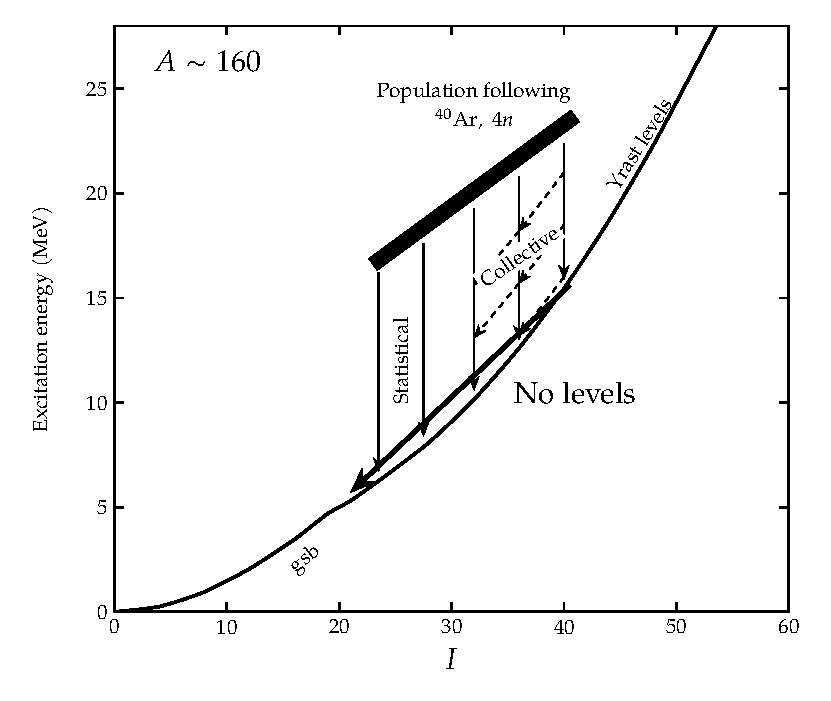
\includegraphics[width=0.7\linewidth]{pictures/3_1}{\small\caption{\label{fig:3.1}{\small 反应($\ce{^{40}Ar},4n$)的激发能-角动量函数关系。在四中子蒸发后，原子核以统计E1和集体E2方式发生$\gamma$级联跃迁，直至晕转线上，而后沿着晕转线发生一系列的E2跃迁。晕转带的强度是逐渐增加的，因为它包含了所有统计跃迁的贡献(\textquotedblleft 边带馈入\textquotedblright )。图片来自文献\cite{SBD77}。}}
} 
\end{figure}

迄今为止，只有这些过程中最后的部分可以被确定为一些分立的线（见3.5节）。通过这种方式所观察到的最大角动量落在$30\hbar$到$40\text{\ensuremath{\hbar}}$之间。目前的测量认为这级联过程的剩余部分是$\gamma$连续的，我们只能从这些实验数据中得到间接的结论{[}GG
67, BSC 75, SBC 76, Di 76, HLM 78, ABH 78, WF 78b{]}。然而，有证据显示沿着平行于晕转线发生的集体跃迁也有着重要的作用；并且在能量高于晕转线几个MeV的地方，集体效应和统计效应存在着竞争{[}SBD
77{]}。

\subsection{晕转带的结构}

在1.7节我们说过一个绕其扁椭球形的对称轴作低角频率转动（Hiskes机制，见图3.2a）下的\emph{经典液滴}\cite{CPS74}。只有在很高的角速度下，原子核会发生相变，并转而由Beringer-Knox机制描述。这种情形下它会发生接近于长椭球形的三轴形变，使得转动轴垂直于其近似的对称轴（见图3.2b）。对于更高的转动频率下，原子核最终会发生衰变（见图3.2c）。

\begin{figure}[H]
\begin{centering}
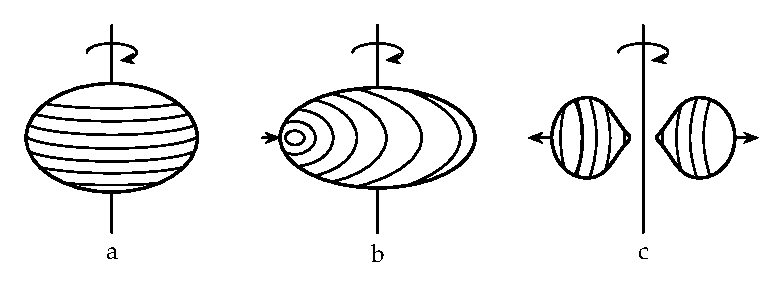
\includegraphics[scale=0.2]{pictures/3_2} 
\par\end{centering}
\caption{\label{fig:3.2}{\small 一个经典液滴在逐渐增长的角速度下的行为}}
\end{figure}

然而，\emph{真实核子}是一个量子力学系统，它表现出壳效应（见2.9节），这使得在元素周期表的某些区域的原子核存在着稳定的基态形变。晕转带对应着每个角动量值的最低能量态；在基态上几十个MeV的激发能全部是转动能量，并且是这些能量产生了角动量。因此，在这条线下的能级密度是很低的，要比在对应能量下$I=0$的能态密度低得多。这个概念类似于基态，然而我们会发现一些对其的典型的偏离。由于核子在晕转区是冷的，我们可以期待其是高度有序的。壳效应起到了重要的作用。

在高角动量下，由壳效应引发的长椭球形变与经典液滴的扁椭球形变具有相同的数量级（见1.7节）。因此当我们研究核子形状与角动量的关系时，我们可以期待在宏观的离心效应与微观的壳结构之间存在的复杂的相互作用。

首先让我们来研究变形良好的重核（例如在稀土区域的元素）的情形。由于壳效应，它们在基态存在着长椭球形的轴对称四极形变。在对应的变形势下，能级由具有相反的单粒子角动量（$\pm\Omega$）的两个核子成对地占领。在第6章我们会看到，就如我们所假设的那样，成对的两个核子不会独立运动，而是由一种配对力耦合在一起——即所谓的自旋为0的Cooper对系统。也就是说，这些形变核会表现出\emph{超流行为}，它们的基态能量也会因此降低几个MeV。

在角动量逐渐增大时，根据晕转带显示出的不同结构，我们可以区分原子核形变的不同机制\cite{BM74}： 
\begin{enumerate}
\item[(a)] 对于较低的角动量量子数$I=0,2,4...$，晕转带与\emph{基态转动带}重合，这在1.5节中已经有过讨论。此时转动是集体的，也就是说转动角速度是与对称轴垂直的（见图3.3a，图中我们已经画出了方向沿着对称轴的Cooper对）。

\begin{figure}[H]
\begin{centering}
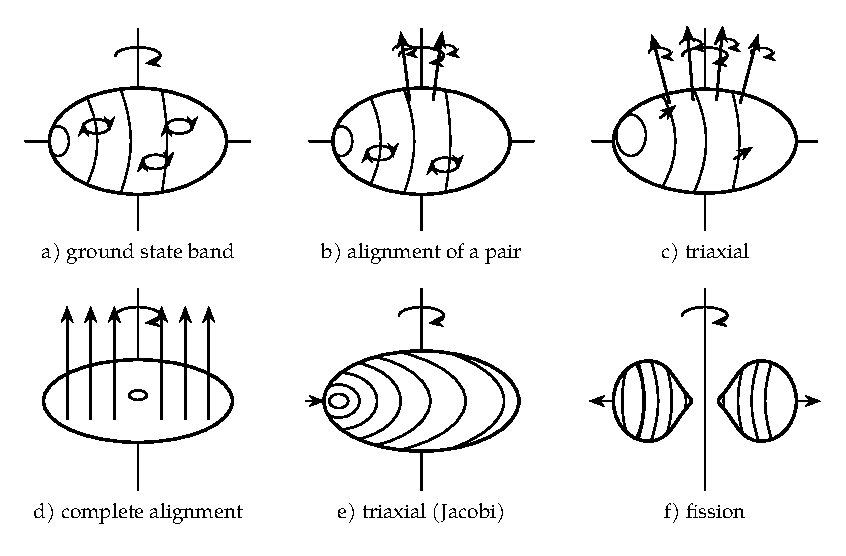
\includegraphics[scale=0.25]{pictures/3_3}\caption{\label{fig:3.3}沿着晕转线形变核的可能结构}
\par\end{centering}
\end{figure}

此时核子处于一个缓慢转动的势场当中（更详细的讨论见3.4节）。对于角动量相反的一对粒子，Coriolis力作用在它们的旋转上，并趋向于让它们的方向与转动轴方向相同，也就是说，Cooper对有被拆开的趋向（\emph{Coriolis拆对效应}；Coriolis
anti-pairing effect, CAP）。然而，在低角动量的情形下，Coriolis力很弱而不足以拆对，原子核将或多或少的与基态时具有相同的结构。

然而我们需要强调的是，在微观图像下，总角动量是由单个核子的角量子数产生的。在集体转动下，这是通过将所有的粒子略微拉向旋转轴方向来实现的。对于每一对粒子而言，这种效应是很小的；粒子对的自旋依然几乎是与势能的对称轴反平行的。当这些小的贡献被累积起来时，我们得到了总角动量$I=2,4...$
\item[(b)] 在角动量逐渐变得越来越大的时候，Coriolis力将变得越来越强，直到大到某一个确定的值时，它将能够拆对。因此在某一个角动量值$I_{c}$时我们可以期待，所有的粒子对都将被拆掉。对关联的消失意味着我们可以观察到一种\emph{相变}，即从超流相向一般相的转变。这种效应在1960年由Mottelson和Valatin所预言\cite{MV60}。
然而更细致的研究表明，Coriolis力的大小是正比于我们所考虑核子的单粒子轨道角动量$j$大小的。在2.8节中我们已经看到，在Fermi面附近的核子分属于不同$j-$值的子壳，而我们期望具有较大$j-$值的那些核子将率先被拉向转动轴的方向。通常，在这样的考虑下，拥有高自旋和相反宇称的能级将在自旋宇称的作用下向下移动，例如稀土元素区的$i_{13/2}$壳层（Stephens-Simon
效应\cite{SS72a}）。

在晕转带的第二种机制之中（见图3.3b），我们可以期待一对或几对已拆对粒子的\emph{顺排过程}，而原子核的其他部分与此同时几乎是不变的。在此之后，晕转带将不再与基态带重合，而是代表着在一个旋转核外存在两个顺排了的粒子体系的能带。两个$i_{13/2}$态的粒子总计能够为转动提供12个单位的角动量。这样的顺排现象的出现是由于，作为集体角速度的函数，角动量$I$的增长是十分迅速的；这会引起能谱上的一些反常效应，例如“回弯现象”（见下）。
\item[(c)] 在平均场的意义上，每一个顺排过程都与集体性质的特定改变联系在一起：被拆的对不再对对关联产生贡献；由于阻塞效应（见6.3.4节），这些关联在若干个顺排过程之后将会完全消失。与旋转轴顺排的粒子的密度分布是一个以旋转轴为对称轴的扁椭球。在与长椭球形的核心结合之后，我们得到了一个三轴形变的混合体。

在晕转带的第三种机制之中（见图3.3c），角动量的大致范围在$30\text{\ensuremath{\lesssim I\lesssim50}}$，我们可以期待Coriolis力与离心力的作用强度能够与壳效应比拟，因此将导致原子核的\emph{三轴形变}。这样的一个没有对称轴的系统要比一个轴对称转子（见1.5.3节）拥有更多的集体态：我们期望存在着平行于晕转带的一系列转动态存在，它们对应着\emph{摆动运动}。
\item[(d)] 如果大多数的核子都与转动轴的方向平行顺排，我们最终得到了一个轴对称的扁椭球。原子核的波函数关于这个轴是转动对称的。转动不再是集体的了；取而代之的是，总角动量是由在变形势阱中不同粒子的重新占据所组成的。

这种运动形式被称为\emph{“单粒子”转动}。在晕转带的这个区域，态的能量是由单粒子能量和转动的扁椭球势阱决定的。相邻态的能量差异会发生统计上的变化。只有在平均意义上，它们符合刚性转子能量的$I(I+1)$定律（见3.4.6节）。从一个态到相邻态的跃迁对应着一次重新占据，并且这矩阵元应该对应着单粒子的值，也就是说这跃迁概率将大幅减少。

由于在晕转带的这个区域能级的统计性特征，我们同时可以期待“高自旋同素异能态”的存在，即所谓的晕阱 \cite{BM74}，这最终会导致延迟衰变的出现，并使我们对整条晕转带级联衰变的观察落在离散的线段上，而不是一个均匀的统计跃迁的背景。
\item[(e)] 在很大角动量的情形下，我们最终期待只有宏观性质是重要的，也就是说，核子应该重复发生扁椭球-三轴-长椭球的形变过程，直至它发生裂变。
\end{enumerate}
迄今为止，只有机制(a)和(b)的离散能级已被观察到；对于剩余区域的很大一部分机制尚处于猜测之中。我们将会在3.4.5节中看到人们曾用以得到这些理论预言的模型。事实上，在计算中我们可以得到上面所讨论的所有机制。

然而，似乎并不是所有原子核都会经历上述的所有阶段。特别是对于小形变或球形核的情况，它们是从机制(d)开始的——也就是说，在发生三轴形变和裂变之前的一个绕着对称轴旋转的扁椭球。另一方面，对于许多大形变的核，在顺排过程中产生的变化不足以补偿其原本长椭球形变所产生的壳效应。在裂变之前它们仅仅会发生三轴形变（见图3.3c与3.3d），而不是扁椭球。在实验上，人们只观测到了作为高自旋同素异能态（晕阱）的小形变原子核，这似乎是与我们的理论符合的。

除了晕转带之外，人们在低自旋和\emph{中自旋区域}观测到了许多其他的转动带。它们的存在基于更加复杂的机制，例如准粒子激发或者是振动态。

在这些机制当中，依赖于$j$壳层轨道的规模，人们可以设想出各种各样的顺排过程。例如在一个奇A核中，在$i_{13/2}$壳上一个奇中子的顺排对应着所谓的\emph{解耦带}。另一个例子是奇奇核中的转动带，此时$i_{13/2}$壳中只有一个中子发生顺排，而质子与对称轴的方向保持一致。这样的带具有一种\emph{半解耦}的结构
\cite{NVR75}。

在3.3节中讨论的粒子加转子模型提供了一种描述这些过程的唯象方法。在那一节中我们将在更细节的程度上讨论以上这些类型的例子。

\subsection{晕转带的唯象描述}

多年来，一些唯象模型被提出来描述转动带的性质和特征。在低自旋区域（见图3.3a），能谱通常符合精确的$I(I+1)$定律；但是对于较大的$I$值，能谱可能发生对这一定律或多或少的偏离\footnote{对于这些数据的一个整合，见 \cite{SHJ73,SSM75}。}。为了描述其与理想的转动谱的偏离，我们通常采取如下的参数化方法：

\begin{equation}
E(I)=A\cdot I\cdot(I+1)+B\cdot(I(I+1))^{2}+C\cdot(I(I+1))^{3}+...
\end{equation}

在很多情况下，这一展开方式的收敛性被证明是相当差的，而一个对\emph{角频率}$\omega$作展开的方法是更合适的。

原则上讲，$\omega$不是一个可以直接测量的量，然而我们可以将其半经典地定义成为

\begin{equation}
\omega=\frac{\text{\ensuremath{\mathrm{d}}}E}{\mathrm{d}J},\text{其中}J=\sqrt{I(I+1)}
\end{equation}

现在将微商用有限差分代替\footnote{这种处理方法不是我们独有的，不同的人会采用不同的处理方法（见\cite{JS74,So73,LR78}）。}，我们可以得到一个“实验”值，\emph{角速度}\footnote{在本章中我们总是使用$\hbar=1$的单位制。}的定义为

\begin{equation}
\omega_{\text{exp}}\simeq\frac{\Delta E}{\Delta\sqrt{I(I+1)}}\bigg|_{I,I-2}\simeq\frac{E(I)-E(I-2)}{\sqrt{I(I+1)}-\sqrt{(I-2)(I-1)}}
\end{equation}

\emph{转动惯量}定义为

\begin{equation}
\mathcal{\mathcal{J}}=\frac{J}{\omega}=\frac{1}{2}\left(\frac{\mathrm{d}E}{\mathrm{d}J^{2}}\right)^{-1}\simeq\frac{2I-1}{\Delta E_{I,I-2}}
\end{equation}

通过这些定义，我们可以计算出晕转带上每一个能级的$\text{\ensuremath{\omega}}$和$\mathcal{J}$的值。
\begin{booknote*}
此时

\[
\mathcal{J}=\frac{J}{\omega}=J\frac{\mathrm{d}J}{\mathrm{d}E}=\frac{1}{2}\left(\frac{\mathrm{d}E}{\mathrm{d}J^{2}}\right)^{-1}
\]
\end{booknote*}
Harris \cite{Ha65a} 提出了如下对能谱的参数化方法：

\begin{equation}
E(I)=\alpha\omega^{2}+\beta\omega^{4}+\gamma\omega^{6}+...
\end{equation}

由于在反向的角速度下，能量$E$不会发生改变，$\omega$的奇数次项不会出现。由于$\omega$是$I$的函数，我们可以选择如(3.3)式中的实验值作为其定义，或者我们也可以定义一个类似上式的转动惯量的展开式，从

\begin{equation}
\frac{\mathrm{d}E}{\mathrm{d}\omega}=\frac{\mathrm{d}E}{\mathrm{d}J}\frac{\mathrm{d}J}{\mathrm{d}\omega}=\omega\frac{\mathrm{d}J}{\mathrm{d}\omega}
\end{equation}

我们可以得到

\[
J(J+1)=\sqrt{I(I+1)}=2\alpha\omega+\frac{4}{3}\beta\omega^{3}+\frac{6}{5}\gamma\omega^{5}+...
\]

当然，这个展开式只有在$J$不是$\omega$的多值函数时才是有效的，也就是说，不在回弯的区域（见3.2.4节）。

另一个被广泛采用来描述转动甚至是过渡性原子核的模型是\emph{可变转动惯量}（variable moment of inertia，VMI）模型
\cite{MSB69,SDG76}。转动惯量$\mathcal{J}$被认为是一个变量，并且有一个内禀的能量$V$依赖于它：

\begin{equation}
E(I,\mathcal{J})=\frac{1}{2\mathcal{J}}I(I+1)+V(\mathcal{J})
\end{equation}

根据变分原理（在5.2中有相关的讨论），对于固定的$I$值，$\mathcal{J}$的取值应该使总能量处于极小值点。这决定了$\mathcal{J}(I)$函数关系。假设我们已知$V(\mathcal{J})$，那么$\mathcal{J}(I)$显然由下式给出

\[
\frac{\mathrm{d}E}{\mathrm{d}\mathcal{J}}\bigg|_{I}=-\frac{1}{\mathcal{J}}\frac{I(I+1)}{2\mathcal{J}}+\frac{\mathrm{d}V}{\mathrm{d}\mathcal{J}}=0
\]

通常我们可以取$V=\frac{1}{2}C(\mathcal{J}-\mathcal{J}_{0})^{2}$，其中$\mathcal{J}_{0}$是在$I=0$处$\mathcal{J}$的取值。系数$C$和$\mathcal{J}_{0}$是从实验能谱$E(I)$拟合得到的。根据关系$J=\omega\cdot\mathcal{J}$，这个模型和Harris模型直至$\omega^{4}$阶是一致的，但(3.7)式的假设显然是更一般的
\cite{DB73,SDG76}。

\subsection{回弯现象}

在10到20个单位角动量的区域，人们在许多核子的晕转带上发现了反常的现象，这现象可以被$\mathcal{J}-\omega^{2}$函数关系图直观地表示出来。在VMI模型的最低阶中（$\mathcal{J}=\mathcal{J}_{0}+b\omega^{2}+...$），这图形应当是一条直线，其对于一个常数的偏离可以作为$I\cdot(I+1)$定律有效性的衡量。图3.4给出了这种曲线的两个例子，由Jülich合作组测得
\cite{LR78}。

\begin{figure}[H]
\centering{}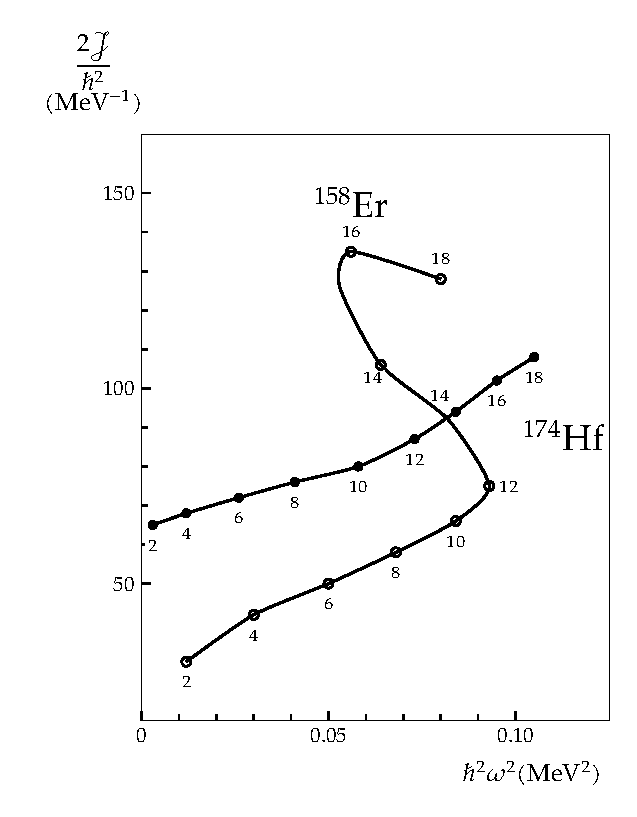
\includegraphics[scale=0.6]{pictures/3_4}\caption{\label{fig:3.4}$^{158}$Er和$^{174}$Hf核的转动惯量-角动量平方的函数图}
\end{figure}

在低自旋的区域我们发现这图形确实是一条直线。对于核$^{174}$Hf，函数对直线的偏离是光滑的。然而对于核$^{158}$Er，在某个特定的$I$值处转动惯量出现了一个都陡峭的上升，甚至使得曲线回弯了（“回弯”现象
\cite{JRH72}）。这在实验上意味着，本应该随着$I$线性增长的跃迁能量$\Delta E_{I,I-2}$

\begin{equation}
\Delta E_{I,I-2}=\frac{1}{2\mathcal{J}}(4I-2)
\end{equation}

不再增大，而是在某一个$I$值开始减小。图3.5给出了与图3.4一致的实验结果。

\begin{figure}[H]
\centering{}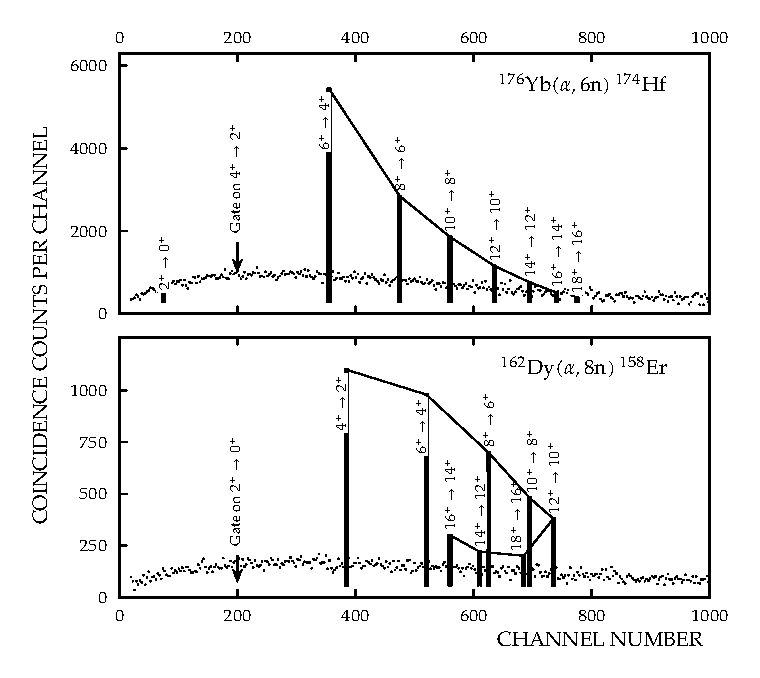
\includegraphics[scale=0.6]{pictures/3_5}\caption{\label{fig:3.5}核反应$^{176}$Yb($\text{\ensuremath{\alpha,6n}}$)$^{174}$Hf和$^{162}$Dy($\text{\ensuremath{\alpha,8n}}$)$^{158}$Er。后一个反应在$I$为$10^{+}-14^{+}$的区域内显示出了名为回弯的反常。为了显示出这种现象，我们用直线将逐渐降低的峰值连接在了一起。}
\end{figure}

这样的现象很容易被两个能带发生交叉的效应所重现（某些情形下我们甚至能够在实验上观测到第二条能带，见图7.6和 \cite{KSM78}）。为了理解这一点，让我们假设两条代表不同转动惯量的曲线在$E-I$图上是两条抛物线。当$\mathcal{J}_{2}>\mathcal{J}_{1}$时，这两条曲线在$I$的某一特定区域会发生交叉。由于剩余相互作用，这样的交叉是不会发生的（不交叉规则，见2.8.4节），因此我们可以得到二阶导数是负的区域，即

\begin{equation}
0>\frac{\mathrm{d}^{2}E}{\mathrm{d}J^{2}}=\frac{\mathrm{d}\omega}{\mathrm{d}J}
\end{equation}

这意味着，随着$\omega$的减小$\mathcal{J}$将变大，同时这两条带的性质将发生交换。事实上，从带混合的观点出发的计算很容易就能解释这样的回弯现象——这样的计算需要包含很少的几个参数，其中一个是两条带之间的相互作用$V$。对于$V$很小的情形，我们会发现一个突兀的转变点，进而发生回弯的现象；而对于$V$较大的情形，转变区域将变得很宽，我们不会再看到回弯现象的出现
\cite{MR72,GG74b}。

\begin{figure}[H]
\centering{}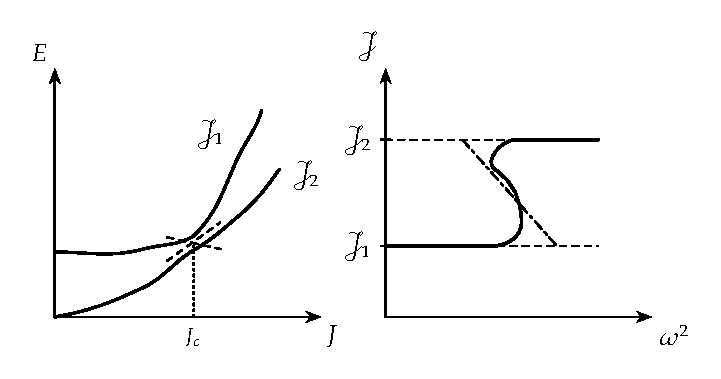
\includegraphics[scale=0.8]{pictures/3_6}\caption{\label{fig:3.6}不同转动惯量曲线$\mathcal{J}_{1}$和$\mathcal{J}_{2}$相互作用的示意图，以及与之对应的回弯现象（取自
\cite{LR78}）}
\end{figure}

另一方面我们很清楚的是，在$\mathcal{J}-\omega^{2}$图形上出现这个奇怪的回弯行为的根源是，我们是在晕转带的一个临界区域探讨问题——我们在背后物理机制不同的两条带之间进行了转换。如果我们只研究基态带的情况，那么对于大$I$值下将不再有晕转带，我们将会得到一条非常平滑的转动惯量关于角速度的曲线（见图3.6中的虚线）。人们经常沿着晕转带研究的原因是其上面的态在实验上是最容易得到的
\begin{comment}
这个问题类似于能级的交叉。对于同一个核，其不同转动机制下的转动惯量曲线很可能存在交叉点，因此使得能量最低的曲线上不止有一种转动惯量的贡献，这种问题似乎可以用最近新出现的本征值延拓方法进行研究——然而对于原本应该交叉之处不交叉的原因，也就是两个“能级”之间的相互作用，暂未有更深层次的理解。此外，能级交叉的现象和相变可能存在着关系。我的理解似乎与下面给出的第一种理论模型相符。
\end{comment}
。

在所有的这些思考之中，我们应该时刻谨记唯象模型只能告诉我们这些能谱的特征，但并不能告诉我们它们背后的物理机制。例如，对于以上讨论的回弯机制，我们可以研究第二条带出现的物理本质。人们已经提出了三种理论解释
\begin{comment}
这三种似乎并非是互斥的；第三种理论解释玄之又玄，我无法理解它描述了怎样的一个物理图像。
\end{comment}
：
\begin{enumerate}
\item 在第二条转动惯量带上，原子核发生了与另一条带不同的形变，例如三轴形变。这意味着回弯现象是由形变的突然改变引起的 \cite{Th73,SV73}。
\item 与基带不同，第二条能带上的状态并不是超流的。这意味着回弯现象是由于从超流体向常规流体相变引发的（Mottelson-Valatin
效应 \cite{MV60}）。
\item 第二条带是由两个绕转动轴转动顺排的准粒子组成的带（见 3.3 节）。此时回弯将对应于一对核子的突然顺排（如 Stephens 和 Simon
所提出 \cite{SS72a}）。
\end{enumerate}
包含所有这些自由度的理论研究（见 7.7 节）的一般结果显示，对于良好形变的核（经典的转子）
\begin{comment}
这里原文直译为“好形变的核”，笔者认为指的应该是形变较为稳定的核。
\end{comment}
，对关联的减少只有在低自旋区会使得转动惯量发生缓慢的增加；但像是回弯一类的突变现象，则是由于一对高 $j$ 轨道核子的顺排而出现的。这种对于回弯现象的解释也有着许多实验上的支持
\cite{GSD73,RSS74,WBB75,SLM76,St76}。

在稀土元素区，$i_{13/2}$ 的中子扮演着重要的角色。然而实验上 \cite{LAD77,BBB79a} 在自旋为 $26\sim30\,\hbar$
\begin{comment}
原文如此，令人怀疑角动量的单位。
\end{comment}
的区域发现了第二个反常现象存在的证据，即所谓的\emph{二次回弯}。这一现象被解释为一对 $h_{11/2}$ 质子的顺排 \cite{FP78}。其他高
$j$ 轨道的核子可能在周期表其他区域的元素中扮演着类似的角色。
\begin{comment}
终此一节，我们在研究唯象模型的解释时将“alignment”译为对齐，在含义上指的是一对核子自旋轴变为了平行方向；然而此译法似不常用。
\end{comment}


\section{粒子加转子模型}

为了描述粒子运动和集体转动之间的相互关系，Bohr 和 Mottelson \cite{BM53} 提出了一个模型：考虑若干近似独立地运动于核心形变势阱中的价粒子，并将它们与一个代表其余粒子的集体转子相耦合。划分价粒子和核心的方式并不总是唯一的。然而一种合理的方式是，在奇
$A$ 核中将未成对的核子视为价核子，而留下一个偶偶核心。我们也可以将粒子-空穴激发的粒子和空穴视为价粒子
\begin{comment}
这里类似壳模型，只不过处理的Hamilton量不太一样。
\end{comment}
。更一般地来讲，我们可以将 Hamilton 量分为两部分：内禀部分 $H_{\text{intr}}$，其在微观层面上描述价粒子或
Fermi 面附近的一整组核子；以及一个用来描述惰性核心的唯象部分 $H_{\text{coll}}$：

\begin{equation}
H=H_{\text{intr}}+H_{\text{coll}}\label{eq:3.10}
\end{equation}

\emph{内禀部分}具有如下形式：

\begin{equation}
H_{\text{intr}}=\sum_{k}\epsilon_{k}a^{\dagger}_{k}a_{k}+\frac{1}{4}\sum_{klmn}\bar{v}_{klmn}a^{\dagger}_{k}a^{\dagger}_{l}a_{n}a_{m}\label{eq:3.11}
\end{equation}

此处 $\epsilon_{k}$ 是形变势中的单粒子能量（例如 Nilsson 能量），而 $\bar{v}$ 是价粒子间的相互作用——在很多情况下这是可以被忽略的。\footnote{我们将在第6章中看到，对关联在形变核中起着重要作用，因此我们应当讨论准粒子而非粒子。这仅给下面给出的公式带来简单的占据因子，出于完整性考虑我们有时会给出这些因子。如欲深入理解，读者可参阅第6章。}

\textit{集体的部分}描述了惰性核心的转动：

\begin{equation}
H_{\text{coll}}=\frac{R^{2}_{1}}{2\mathcal{J}_{1}}+\frac{R^{2}_{2}}{2\mathcal{J}_{2}}+\frac{R^{2}_{3}}{2\mathcal{J}_{3}}\label{eq:3.12}
\end{equation}
其中 $R_{i}$ 是核心集体角动量在体固坐标系中的分量。它与价粒子的角动量 $\boldsymbol{j}$（即各单粒子角动量之和）共同构成了总角动量
$\boldsymbol{I}$（参见附录 A）：

\begin{equation}
\boldsymbol{I}=\boldsymbol{R}+\boldsymbol{j}\label{eq:3.13}
\end{equation}
消去 $\boldsymbol{R}$ 后，$H_{\text{coll}}$ 可以分解为三部分：

\begin{equation}
H_{\text{coll}}=H_{\text{rot}}+H_{\text{rec}}+H_{\text{cor}}\label{eq:3.14}
\end{equation}
其中

\begin{equation}
H_{\text{rot}}=\frac{I^{2}_{1}}{2\mathcal{J}_{1}}+\frac{I^{2}_{2}}{2\mathcal{J}_{2}}+\frac{I^{2}_{3}}{2\mathcal{J}_{3}}\label{eq:3.15}
\end{equation}
是转子的纯转动算符{[}式 (1.55){]}，它仅作用于转子的自由度，即 Euler 角。项

\begin{equation}
H_{\text{rec}}=\sum^{3}_{i=1}\frac{j^{2}_{i}}{2\mathcal{J}_{i}}\label{eq:3.16}
\end{equation}
通常被称为\emph{反冲项}（recoil term）。它代表转子的反冲能量。该算符仅作用于价粒子的坐标空间。对于多个价粒子的情形，它包含两体相互作用。

最后，Coriolis 相互作用

\begin{equation}
H_{\text{cor}}=-\sum^{3}_{i=1}\frac{I_{i}j_{i}}{\mathcal{J}_{i}}\label{eq:3.17}
\end{equation}
将价粒子的自由度与转子的自由度耦合在一起。这种纯粹的运动学耦合是该模型中唯一的耦合作用。

应当注意到，实验室坐标系中的总角动量算符 $I_{x},I_{y},I_{z}$ 与 Hamilton 量 \ref{eq:3.10}
对易。尽管在内禀参考系中转动对称性受到了破坏（例如在 Nilsson Hamilton 量中），但该模型对于全系统仍然保持角动量守恒，这是因为算符
$I_{x},I_{y},I_{z}$ 仅作用于 Euler 角，并与内禀分量 $I_{1},I_{2},I_{3}$ 对易（参见附录
A）。然而必须强调的是，这种转动不变性仅仅是通过引入唯象的核心才得以实现的。如果人们希望微观地处理所有粒子（即核心消失的极限），Euler
角就成了冗余变量（参见 11.3 节）。

系统的波函数可以写为

\begin{equation}
|\Psi^{I}_{M}\rangle=\sum_{K}\Phi_{K}|IMK\rangle\label{eq:3.18}
\end{equation}
其中 $\Phi_{K}$ 依赖于价粒子的坐标，而 $|IMK\rangle$ 依赖于 Euler 角，并在式 (A.21) 中定义。在最简单的特定情形下，体系仅包含一个价粒子与一个轴对称转子。利用该模型，人们极其精确地重现了奇
$A$ 核的大量实验能谱；从这一角度来看，它无疑是核物理中最有力的模型之一。然而，迄今为止该模型仍缺乏严密的微观推导。这样一个推导应当从多体
Hamilton 量 (2.19) 出发，将 $3A$ 个粒子坐标以适宜的方式变换为 $3A-3$ 个内部坐标以及描述集体运动的
3 个 Euler 角。与该变换相对应，Hamilton 量应分解为内部部分与集体部分，正如\ref{eq:3.10} 所示。最终，人们希望利用形变壳模型来描述内部运动。

人们在这一方向上做出了许多尝试，我们在 11.3 节中对此给出了简要讨论，但直到目前该问题仍未得到彻底解决。对于良好形变核的情形，该模型可以由以下论据提供支持：
\begin{enumerate}
\item[(i)] 微观 Hartree-Fock 计算在轴对称形变处展现出非常显著的能量极小值，这证实了转动核心概念的合理性。
\item[(ii)] 该模型在一定程度上等价于 cranking 模型（参见 3.4 节），后者至少在强轴对称形变极限下具有微观基础。
\item[(iii)] Villars 和 Cooper \cite{VC70} 证明，在引入冗余坐标后，可以得到类似于\ref{eq:3.10} 形式的
Hamilton 量，不过带有额外的耦合项。在强形变极限并引入进一步假设的前提下，他们得到了正确的转动惯量表达式。
\end{enumerate}
然而，粒子加转子模型也被非常成功地应用于小形变区以及过渡核中。目前尚不清楚这一成功如何从微观上予以解释。

\subsection{轴对称情形}

假设转子以 3 轴为对称轴，即 $\mathcal{J}_{1}=\mathcal{J}_{2}=\mathcal{J}$，此时不可能存在绕该轴的集体转动，因而
$\boldsymbol{R}$ 的 3 分量必须为零（参见 1.5 节）。由\ref{eq:3.13} 立即得到，总角动量 $\boldsymbol{I}$
的 3 分量 $K$ 必定等于 $\boldsymbol{j}$ 的 3 分量 $\Omega$：

\begin{equation}
K=\Omega\label{eq:3.19}
\end{equation}
对于 Hamilton 量 \ref{eq:3.10}、\ref{eq:3.14} 中的各项，在此情形下我们得到：

\begin{equation}
H_{\text{intr}}=\sum_{i,\Omega}\epsilon^{i}_{\Omega}a^{\dagger}_{i\Omega}a_{i\Omega}\label{eq:3.20}
\end{equation}

\begin{equation}
H_{\text{rot}}=\frac{\boldsymbol{I}^{2}-I^{2}_{3}}{2\mathcal{J}}\label{eq:3.21}
\end{equation}

\begin{equation}
H_{\text{rec}}=\frac{1}{2\mathcal{J}}\left(j^{2}_{1}+j^{2}_{2}\right)\label{eq:3.22}
\end{equation}

\begin{equation}
H_{\text{cor}}=-\frac{1}{\mathcal{J}}\left(I_{1}j_{1}+I_{2}j_{2}\right)=-\frac{1}{2\mathcal{J}}\left(I_{+}j_{-}+I_{-}j_{+}\right)\label{eq:3.23}
\end{equation}
在\ref{eq:3.20} 中我们忽略了剩余相互作用。轴对称势阱中的单粒子能级由量子数 $k=(i,\Omega)$ 标记，对应的本征函数记为
$\Phi^{i}_{K}$。

反冲项仅作用于内禀坐标。它经常被忽略，因为内禀单粒子能量 $\epsilon^{i}_{\Omega}$ 通常是根据实验数据进行拟合调节的。在接下来的讨论中我们遵循这一论据，暂且略去
$H_{\text{rec}}$。直到 3.3.2.1 节我们才会重新讨论它。Hamilton 量 \ref{eq:3.20}–\ref{eq:3.23}
具有\ref{eq:3.18} 类型的本征函数，这可以通过对 Hamilton 量 \ref{eq:3.10} 进行数值对角化求得。然而，\ref{eq:3.20}–\ref{eq:3.23}
中各项的重要性取决于具体的物理情境。因此，考察以下三种极限是非常有益的；在这些极限中某一项占据主导地位，从而使问题能够解析求解（综述参见
\cite{St75a}）：

在\emph{强耦合极限}下，奇粒子绝热地跟随偶偶核心的转动。当与形变的耦合远强于 Coriolis 相互作用对单粒子运动的微扰时，该极限得以实现。

在\emph{弱耦合极限}下（对应于极小的形变），奇粒子基本上运动于球形壳模型能级上，仅受到微弱的扰动（例如来自四极振动的扰动，参见第
8 章）。

在\emph{解耦极限}下，Coriolis 力非常强烈，以至于与核心形变的耦合可以忽略。此时总角动量与单粒子角动量彼此平行。

\subsubsection{强耦合极限（形变顺排）}

当 Coriolis 相互作用矩阵元与形变壳模型中不同 $\Omega$ 值的单粒子能量能级分裂相比非常微小时，强耦合极限得以实现。我们预期在以下情况下满足该条件：
\begin{enumerate}
\item[(i)] 大形变 $\beta$ 的情形，因为 Nilsson Hamilton 量中的能级分裂正比于 $\beta$，而根据简易经验规则{[}式
(1.50){]}，转动常数 $\hbar^{2}/(2\mathcal{J})\propto\beta^{-2}$；
\item[(ii)] Coriolis 矩阵元很小的微扰情形。正如我们在\ref{eq:3.33} 中将看到的，它们正比于 $[I(I+1)-K(K+1)]^{1/2}[j(j+1)-\Omega(\Omega+1)]^{1/2}$，这意味着在低自旋
$I$ 或处于小粒子角动量 $j$ 轨道的核子情况下该矩阵元很小。对于大的 $j$ 值，只有在很大的 $\Omega$ 值下它们才可以被忽略。
\end{enumerate}
这一极限被称为强耦合或\emph{形变顺排}（deformation aligned）极限，因为在这种情况下 $K$ 是一个好量子数。价粒子的角动量
$\boldsymbol{j}$ 强烈耦合到核心的运动上。在半经典图像中，$\boldsymbol{j}$ 绕 3 轴进动，如\ref{fig:3.7}a
的耦合方案所示。由于 $H_{\text{cor}}$ 是 Hamilton 量中耦合粒子与转子自由度的唯一项，在这一极限下本征函数是函数
$\Phi_{K}$（$H_{\text{intr}}$ 的本征函数，例如单粒子 Nilsson 函数）与对称转子本征函数 $|IMK\rangle$
的直积（参见附录 A）。

\begin{figure}[H]
\begin{centering}
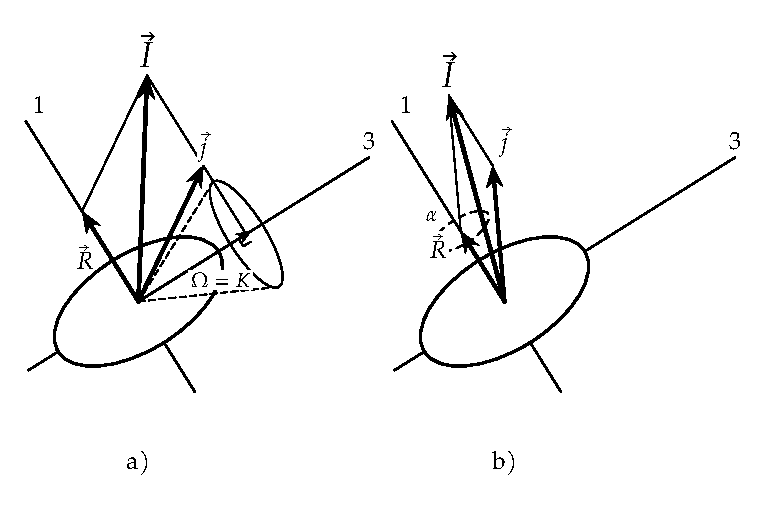
\includegraphics[width=0.7\textwidth]{pictures/3_7}
\par\end{centering}
\caption{\label{fig:3.7}粒子加转子模型中的耦合方案：(a) 强耦合；(b) 转动顺排。}
\end{figure}

我们在 1.5.1 节中已经看到，Hamilton 量 \ref{eq:3.10} 具有额外的对称性 $\mathcal{R}_{1}$，它描述了核心绕体固坐标系
1 轴转动 $180^{\circ}$ 的操作：

\begin{equation}
\mathcal{R}_{1}=\mathrm{e}^{\mathrm{i}\pi R_{1}}=\mathrm{e}^{\mathrm{i}\pi I_{1}}\mathrm{e}^{-\mathrm{i}\pi j_{1}}\label{eq:3.24}
\end{equation}
因此我们必须对波函数 \ref{eq:3.18} 进行对称化，结合式 (A.24) 得到如下本征函数集合 \cite{Ke56}：

\begin{equation}
|\Psi^{I}_{MK}\rangle=\frac{1}{\sqrt{2(1+\delta_{K0})}}\left\{ \Phi^{i}_{K}|IMK\rangle+(-)^{I}\mathrm{e}^{-\mathrm{i}\pi j_{1}}\Phi^{i}_{K}|IM-K\rangle\right\} \label{eq:3.25}
\end{equation}
如果我们已知 $\Phi^{i}_{K}$ 在 $\boldsymbol{j}^{2}$ 本征态上的展开：

\begin{equation}
|\Phi^{i}_{K=\Omega}\rangle=\sum_{nj}C^{i}_{nj}|nj\Omega\rangle\label{eq:3.26}
\end{equation}
我们便发现

\begin{equation}
\mathrm{e}^{-\mathrm{i}\pi j_{1}}|\Phi^{i}_{K=\Omega}\rangle=\sum_{nj}C^{i}_{nj}(-)^{-j}|nj-\Omega\rangle\label{eq:3.27}
\end{equation}
与\ref{eq:3.25} 相对应的能谱由下式给出：

\begin{equation}
E^{i}_{K}(I)=\epsilon^{i}_{K}+\frac{1}{2\mathcal{J}}\left(I(I+1)-K^{2}\right)\label{eq:3.28}
\end{equation}
{[}在\ref{eq:3.28} 中，通常用准粒子能量 $E^{i}_{K}$ 代替 $\epsilon^{i}_{K}$，其定义见式
(6.72){]}。这是转动带的能谱。最低可能的自旋为 $I_{0}=K$。带头能量 $E^{i}_{K}(I_{0})$ 并不严格等于
$\epsilon^{i}_{K}$，而是有微小的位移，尤其是当我们计入反冲项与剩余相互作用时。该能谱具有能级间距 $\Delta I=1$，其转动惯量即为转子的转动惯量。

在这一强耦合极限下，我们完全忽略了 Coriolis 相互作用。若至少在一阶微扰论下计入它，我们仅在 $K=1/2$ 的能带中获得修正：

\begin{equation}
E^{i}_{K=1/2}(I)=\epsilon^{i}_{K=1/2}+\frac{1}{2\mathcal{J}}\left\{ I(I+1)-\frac{1}{4}+a^{i}\left(I+\frac{1}{2}\right)(-)^{I+1/2}\right\} \label{eq:3.29}
\end{equation}
其中所谓的\emph{解耦因子}（decoupling factor）由下式给出：

\begin{equation}
a^{i}=\mathrm{i}\langle\Phi^{i}_{1/2}|j_{+}\mathrm{e}^{-\mathrm{i}\pi j_{1}}|\Phi^{i}_{1/2}\rangle\label{eq:3.30}
\end{equation}
或者若 $\Phi^{i}_{K}$ 具有\ref{eq:3.26} 的形式：

\begin{equation}
a^{i}=-\sum_{nj}|C^{i}_{nj}|^{2}(-)^{j+1/2}\left(j+\frac{1}{2}\right)\label{eq:3.31}
\end{equation}
这意味着，例如对于正的解耦因子（主要成分具有半整数 $j+\frac{1}{2}$ 为奇数），具有 $I+\frac{1}{2}$
为奇数的能级（$I=\frac{1}{2},\frac{5}{2},\frac{9}{2},\dots$）向下移动。这极好地解释了许多核中
$K=1/2$ 能带出现的相当严重的交错扭曲现象 \cite{ABH56}；事实上在这些核中，具有 $\Delta I=2$
的两条分支带（$I+\frac{1}{2}$ 的偶数与奇数值）彼此相对位移。导致这种解耦的原因来自波函数关于 $\mathcal{R}_{1}$
对称化的\ref{eq:3.25}，它通过 Coriolis 矩阵元混合了 $K=1/2$ 与 $K=-1/2$ 的态。解耦因子
$a^{i}$ 的强度取决于对单粒子波函数 $\Phi^{i}_{1/2}$ 有贡献的 $j$ 分量。如果涉及具有大单粒子角动量的能级，解耦因子将非常巨大。然而在这些情况下微扰论不再成立，Coriolis
算符的其他矩阵元也会参与进来。因此，强耦合极限不再能实现，我们必须考虑不同的极限情形。

\subsubsection{弱耦合极限（无顺排）}

如前所述，当 Coriolis 矩阵元在属于不同 $K$ 值的单粒子能级之间引起强混合时，强耦合近似便失效了。因此让我们更详细地研究
Coriolis 矩阵元：

\begin{equation}
\langle\Psi^{I}_{MK+1}|H_{\text{cor}}|\Psi^{I}_{MK}\rangle=-\frac{1}{\mathcal{J}}\sqrt{I(I+1)-K(K+1)}\,\langle\Phi_{\Omega+1}|j_{x}|\Phi_{\Omega}\rangle\label{eq:3.32}
\end{equation}
若 $\Phi_{\Omega}$ 具有\ref{eq:3.26} 所示的形式，我们得到

\begin{equation}
\langle\Psi^{I}_{MK+1}|H_{\text{cor}}|\Psi^{I}_{MK}\rangle=-\frac{1}{2\mathcal{J}}\sum_{nj}|C_{nj}|^{2}\sqrt{I(I+1)-K(K+1)}\sqrt{j(j+1)-\Omega(\Omega+1)}\label{eq:3.33}
\end{equation}
我们看到，当 $I/K$ 与 $j/\Omega$ 很大时，这些矩阵元非常大。也就是说，当涉及具有大 $j$ 与小 $\Omega$
值的能级时便属于此情形。处于这些能级中的粒子具有高角动量，其密度分布紧贴 3 轴。因此显而易见，核心垂直于该轴的转动会对这些粒子的运动产生巨大的影响。

一个著名的例子是中子 $1i_{13/2}$ 能级，在轻稀土核（如 Dy 和 Er）中它位于 Fermi 面附近。人们可以估计在
$\Omega=1/2$ 情形下 Coriolis 矩阵元约为 $0.1\times I\,\text{MeV}$，与 $H_{\text{intr}}$
的能级间距相比这实际上是相当大的。由于这些具有高 $j$ 值的能级被壳模型的自旋-轨道耦合项（参见 2.4 节）极大地向下压入具有不同主量子数
$N$ 的壳层中，这些能级具有相当纯的组态，即 $C_{nj}\simeq1$（闯入态，intruder state）。因此在接下来的讨论中，仅考虑这样一个单独的
$j$ 壳层就足够了。$1i_{13/2}$ 壳层并不是唯一的特例。每个主壳层中具有最大 $j$ 值的能级能量都被急剧拉低，并在许多转动能谱中扮演着极其重要的角色。

Vogel \cite{Vo70} 提出了一个极限（通常称为\emph{弱耦合}或\emph{无顺排}极限），其中 $H_{\text{intr}}$
的 $K$ 分裂被完全忽略。（当然，这只有在极小形变下才是有效的近似。）此时 $\boldsymbol{j}^{2}$ 与 $\boldsymbol{R}^{2}$
均与 $H_{\text{intr}}$ 对易，我们可以构造 $\boldsymbol{R}^{2}$ 与 $R_{3}$ 的共同本征函数（后者的本征值自然为零）。适当的角动量耦合给出\footnote{由于我们将角动量 $\boldsymbol{j}$ 与 $-\boldsymbol{I}$ 耦合为 $\boldsymbol{R}=\boldsymbol{I}-\boldsymbol{j}$，我们必须采用反相位的耦合规则，参见附录
A。}：

\begin{equation}
|\Psi^{IR}_{M}\rangle=\sum_{K}(-)^{j-K}C^{I\quad j\quad R}_{K\ -K\ 0}\Phi_{K}|IMK\rangle\label{eq:3.34}
\end{equation}
这些波函数对角化了 $\boldsymbol{R}^{2}$，对应的能谱形式为

\begin{equation}
E(I)=E_{\text{intr}}+\frac{1}{2\mathcal{J}}R(R+1)\label{eq:3.35}
\end{equation}
满足

\begin{equation}
|j-R|\leqslant I\leqslant j+R;\quad R=0,2,4,\dots\quad(\mathcal{R}_{1}\ \text{对称性})\label{eq:3.36}
\end{equation}
这意味着对于转子的每一个转动量子数 $R$，$\boldsymbol{j}$ 可以有 $2j+1$ 种不同的空间取向而不改变系统的能量（零耦合）。这
$2j+1$ 个能级的分裂可以在一阶微扰论下予以考虑（我们采用 Nilsson 项 $\sim\beta r^{2}Y_{20}$
作为微扰）：

\begin{equation}
E(I)=E_{0}+\frac{1}{2\mathcal{J}}R(R+1)-\beta\hbar\omega_{0}\langle\Psi^{IR}_{M}|r^{2}Y_{20}|\Psi^{IR}_{M}\rangle\label{eq:3.37}
\end{equation}
对应于 $\boldsymbol{j}$ 的每一种取向，都存在核心的一整条具有 $\Delta R=2$ 的转动带。在给定的能量下（即给定的
$R$），具有最高 $I$ 值的能级 $I=R+j$ 对应于晕能级（yrast levels）。这些能级之间由强 $E2$
跃迁相连接 \cite{Re75a}，并在实验上最容易被观测到。它们被称为\emph{优选态}（favored states）\footnote{具有较低顺排程度的能级（例如 $I=j+R-1$）被称为非优选态（unfavored states）。}
\cite{St75a}，其能量由下式给出：

\begin{equation}
E(I)=E_{\text{intr}}+\frac{1}{2\mathcal{J}}(I-j)(I-j+1)\label{eq:3.38}
\end{equation}
这意味着这些态位于一条在 $I=j$ 处具有极小值的抛物线上，这在实验上得到了广泛的证实，\ref{fig:3.8} 给出了一个典型范例。

\begin{figure}[H]
\begin{centering}
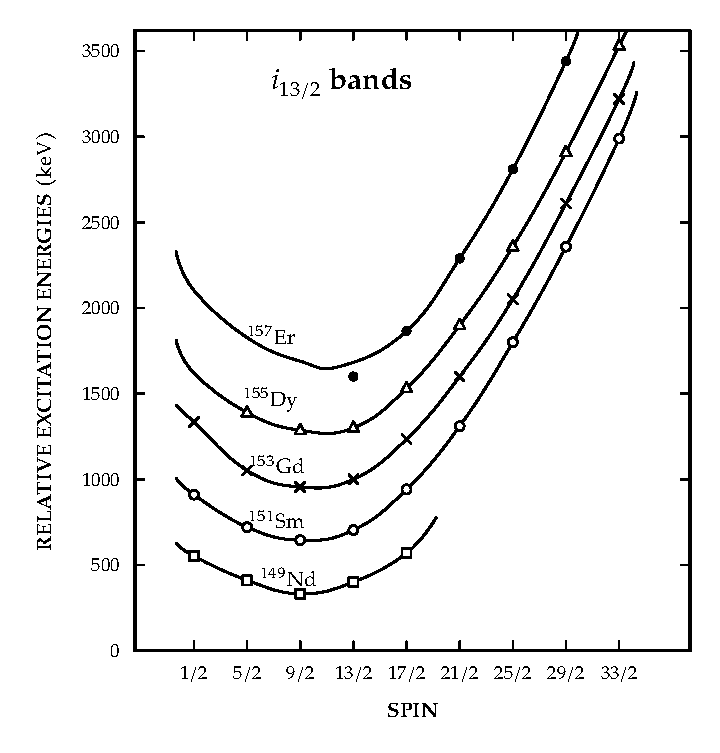
\includegraphics[width=0.75\textwidth]{pictures/3_8}
\par\end{centering}
\caption{\label{fig:3.8}某些 $N=89$ 核中 $1i_{13/2}$ 带的相对激发能随自旋的变化关系。（实验观测到的能带成员在绘制时将
$13/2^{+}$ 态等间距平移（300 keV）。引自 \cite{LR76}。）}
\end{figure}

在这条抛物线的右支上，$\boldsymbol{j}$ 与 $\boldsymbol{R}$ 相互顺排（$\boldsymbol{j}\parallel\boldsymbol{R}$）：

\[
I=j+R=j,j+2,j+4,\dots
\]
而在抛物线的左支上，$\boldsymbol{j}$ 与 $\boldsymbol{R}$ 反向顺排（$\boldsymbol{j}\parallel-\boldsymbol{R}$）；核心的转动方向与
$\boldsymbol{j}$ 相反\footnote{原则上也存在具有 $R>j$ 的反向顺排态 \cite{PO78}。}：

\[
I=j-R=j-2,j-4,\dots,\frac{1}{2}\left(\text{或 }0\right)
\]
作为一条经验规则，弱耦合极限严格来说仅在非常小的形变 $|\beta A^{1/3}|<4$ 下才成立。然而我们将在下一小节看到，即使在更强的形变下（此时忽略
$H_{\text{intr}}$ 的 $\Omega$ 依赖性已不再合理），满足 $\boldsymbol{I}\parallel\boldsymbol{j}$
的态在能量上仍然是极其有利的。因此，在所谓转动顺排耦合方案中，\ref{eq:3.38} 对于更大形变核中的许多能级同样适用（例如参见\ref{fig:3.8}）。

\subsubsection{解耦极限（转动顺排）}

在处于中等形变的情形下，Hamilton 量内禀部分的能级分裂不再能够被忽略。此时外层大 $j$ 粒子的取向不再独立于核心的运动。Stephens
等人 \cite{SDN73} 认识到，若外层粒子沿着长椭球核的转动轴顺排，则单粒子密度分布（主要集中在垂直于 $\boldsymbol{j}$
的平面内）与核心之间的最大重叠要求便能够得到满足（参见 2.8.4 节）。

在数学上，我们可以在单一 $j$ 壳层模型中理解这一点（$C_{nj}\simeq1$，例如在 $1i_{13/2}$ 情形下）。忽略
$\boldsymbol{l}^{2}$ 与 $\boldsymbol{l}\cdot\boldsymbol{s}$ 项，Nilsson
能量简单地由对角矩阵元给出：

\begin{align}
\epsilon_{\Omega} & =\epsilon_{0}-\beta\hbar\omega_{0}\langle nlj\Omega|r^{2}Y_{20}|nlj\Omega\rangle\nonumber \\
 & =\epsilon_{0}+\beta k\frac{3\Omega^{2}-j(j+1)}{4j(j+1)}=\epsilon_{0}-\frac{1}{4}\beta k+C\Omega^{2}\label{eq:3.39}
\end{align}
其中 $k$ 与 $C$ 均不依赖于 $\Omega$。同样，反冲项 \ref{eq:3.22} 可以作为对角矩阵元计算，给出

\begin{equation}
H_{\text{rec}}=\frac{1}{2\mathcal{J}}\left(j(j+1)-\Omega^{2}\right)\label{eq:3.40}
\end{equation}
因此，在此近似下 Hamilton 量 \ref{eq:3.10} 具有形式：

\begin{equation}
H=\epsilon_{0}-\frac{1}{4}\beta k+\frac{1}{2\mathcal{J}}\left(I(I+1)+j(j+1)\right)+\left(C-\frac{1}{2\mathcal{J}}\right)\Omega^{2}+H_{\text{cor}}\label{eq:3.41}
\end{equation}
在特定的形变区域，当 $C\simeq1/(2\mathcal{J})$ 时，来自 Hamilton 量内禀部分与转动部分的 $\Omega$
依赖性恰好相互抵消！事实证明，这一相消对于相当宽广的中等形变区域都适用。遗憾的是，求解\ref{eq:3.41} 所需的 $H_{\text{cor}}$
的本征函数在一般情形下无法解析给出。因此我们在此给出定性的讨论。将 Coriolis 项写作\footnote{$\boldsymbol{I}_{\perp}$ 与 $\boldsymbol{j}_{\perp}$ 分别是 $\boldsymbol{I}$
与 $\boldsymbol{j}$ 垂直于对称轴的分量。}：

\begin{equation}
H_{\text{cor}}=-\frac{1}{\mathcal{J}}\boldsymbol{I}_{\perp}\cdot\boldsymbol{j}_{\perp}\label{eq:3.42}
\end{equation}
我们看到，对于满足 $\langle\boldsymbol{I}\rangle\parallel\langle\boldsymbol{j}\rangle$
的波函数，它的期望值最低。由于 $\boldsymbol{R}$ 垂直于 3 轴，对于单粒子角动量沿垂直于对称轴的转动轴顺排的波函数，我们获得最低的本征值。为此，我们选取
1 轴，并相应地通过将 $j_{3}$ 的本征函数 $|\Phi^{j}_{K}\rangle$ 绕 2 轴旋转 $90^{\circ}$，构造具有本征值
$\alpha$ 的 $j_{1}$ 的本征函数 $|\tilde{\Phi}_{\alpha}\rangle$：

\begin{equation}
|\tilde{\Phi}_{\alpha}\rangle=\sum_{K}d^{j}_{K\alpha}\left(-\frac{\pi}{2}\right)|\Phi^{j}_{K}\rangle\label{eq:3.43}
\end{equation}
其中 $d^{j}_{K\alpha}$ 是该转动的 Wigner 函数 \cite{Ed57}。

然而对于总波函数而言，构造使 $\alpha$ 成为好量子数的态并不那么容易。尝试波函数

\begin{equation}
|\Psi^{I\ j}_{M\ \alpha}\rangle=\sum_{K}d^{j}_{K\alpha}\left(-\frac{\pi}{2}\right)\Phi^{j}_{K}|IMK\rangle\label{eq:3.44}
\end{equation}
至少在 $I\gg K$ 时是 $H_{\text{cor}}$ 的本征函数。由

\begin{equation}
I_{-}|IMK\rangle=\sqrt{I(I+1)-K(K+1)}|IMK+1\rangle\simeq I|IMK+1\rangle\label{eq:3.45}
\end{equation}
我们随即容易得到

\begin{equation}
H_{\text{cor}}|\Psi^{I\ j}_{M\ \alpha}\rangle=-\frac{1}{\mathcal{J}}I\alpha|\Psi^{I\ j}_{M\ \alpha}\rangle\quad(I\gg K)\label{eq:3.46}
\end{equation}
这表明 $\alpha$ 即为 $\boldsymbol{j}$ 在 $\boldsymbol{I}$ 上的投影。

由式 (A.24) 以及 \cite[式 (4.2.4)]{Ed57}，我们得到

\begin{equation}
\mathcal{R}_{1}|\Psi^{I\ j}_{M\ \alpha}\rangle=(-)^{I-\alpha}|\Psi^{I\ j}_{M\ \alpha}\rangle\label{eq:3.47}
\end{equation}
这意味着为了满足对称性条件 $\mathcal{R}_{1}=1$，$I-\alpha$ 必须为偶数。

在 $C\simeq1/(2\mathcal{J})$ 的情形下，对于 Hamilton 量 \ref{eq:3.41} 的能谱我们发现：

\begin{align}
E(I,\alpha) & =\text{const.}+\frac{1}{2\mathcal{J}}\left(I(I+1)+j(j+1)-2I\alpha\right)\nonumber \\
 & =\text{const.}+\frac{1}{2\mathcal{J}}(I-\alpha)(I-\alpha+1)\label{eq:3.48}\\
 & =\text{const.}+\frac{1}{2\mathcal{J}}R(R+1)\label{eq:3.49}
\end{align}
其中根据对称性条件 \ref{eq:3.47}，$R=I-\alpha=0,2,4,\dots$ 必须为偶数。

因此，能量最低的态是那些具有最大顺排的态（$\alpha=j$，优选态）。这完全对应于价核子的自旋取向垂直于 3 轴、而核心完全解耦并以
$R=I-\alpha$ 转动的物理图像；它给出了间距为 $\Delta I=2$ 的能谱，但在其他方面与邻近偶偶核的转动谱完全等价。例如在弱形变核中已经观测到了这类能带（参见\ref{fig:3.8}
与\ref{fig:3.9}）。

\begin{figure}[H]
\begin{centering}
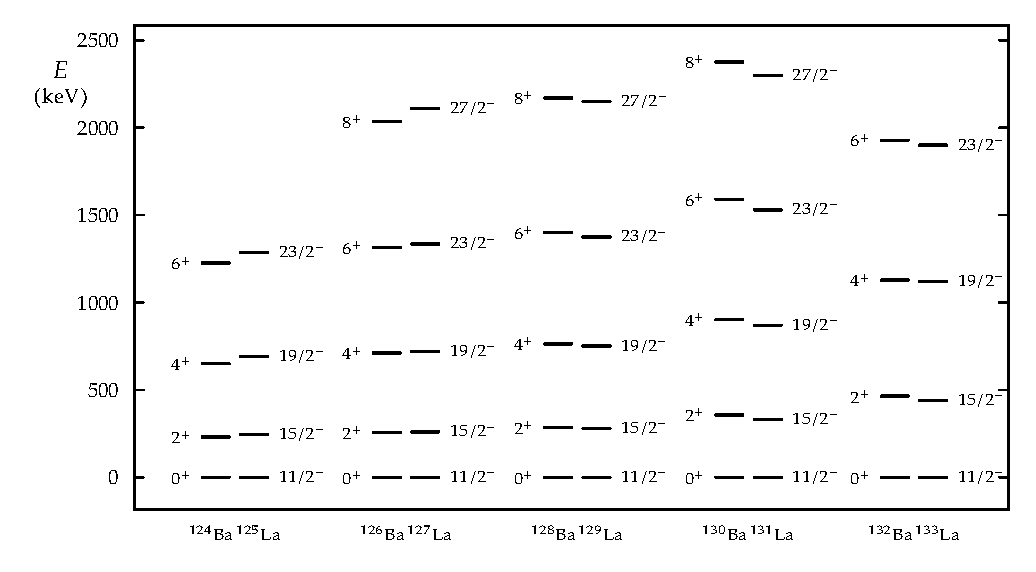
\includegraphics[width=0.75\textwidth]{pictures/3_9}
\par\end{centering}
\caption{\label{fig:3.9}某些 Ba 同位素中的基带能级与邻近 La 核中负宇称带能级的比较。在大多数情况下，La 的 $11/2^{-}$
能级并非基态，其能量已从该核展示的所有能级中扣除。（引自 \cite{St75a}。）}
\end{figure}

顺排程度较低的态（非优选态）具有 $\alpha=j-1$。它们通常位于更高的能量处，因而在 $(\text{HI},xn)$
重离子反应中不会被布居。

\ref{fig:3.10} 给出了轴对称粒子加转子模型中一个位于 $1h_{11/2}$ 壳层的价核子本征值随形变 $\beta$
变化的精确解。对于极小的 $\beta$ 值，呈现出若干近简并多重态的弱耦合方案。在扁椭球一侧（$\beta<0$），强耦合方案得以实现。在此情形下，Nilsson
方案（参见图 2.21）中能量最低的能级是 $\Omega=11/2$ 能级。它的 Coriolis 矩阵元非常微小，因而观测到具有
$\Delta I=1$ 的强耦合带。在长椭球一侧情况则完全相反：能量最低的能级具有 $\Omega=1/2$ 以及巨大的 Coriolis
矩阵元。此时晕带（具有最高 $I$ 值的能级）由具有 $\Delta I=2$ 的解耦带 $I=11/2,15/2,19/2,\dots$
构成，其能级间距与转子的能级间距大致相同（正如在 $\beta=0$ 处所见）。我们还看到，对于这些完全顺排的晕能级，转动顺排耦合方案在相当宽广的中等
$\beta$ 值范围（$0.13\lesssim\beta\lesssim0.23$）内都实现得非常好。只有在极大形变下才会出现显著偏离。

\begin{figure}[H]
\begin{centering}
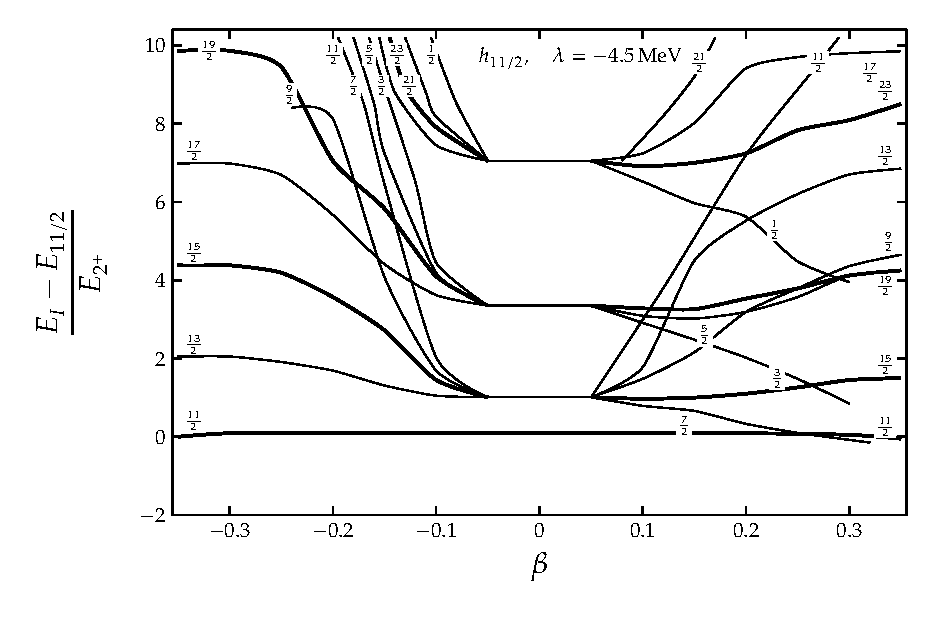
\includegraphics[width=0.75\textwidth]{pictures/3_10}
\par\end{centering}
\caption{\label{fig:3.10}轴对称粒子加转子模型中一个粒子处于 $1h_{11/2}$ 壳层的本征值随形变 $\beta$
的变化关系。图中绘制的是相对于 $I=11/2$ 能级的激发能。Fermi 面 $\lambda$ 位于整个 $1h_{11/2}$
轨道之下。（引自 \cite{St75a}。）}
\end{figure}

当然，能带的结构也依赖于 Fermi 面的位置。在此我们讨论的是壳层中仅有一个粒子的最简单情形。完全类似的情况是高 $j$ 壳层中仅有一个空穴。此时情况颠倒过来：在长椭球一侧是具有大
$\Omega$ 值的能级——即观测到强耦合方案；而在扁椭球一侧是具有小 $\Omega$ 值的能级，表现为解耦方案。

这些思考表明，基于此类高 $j$ 能级建立的转动带结构，为在过渡区通过实验区分长椭球形变与扁椭球形变提供了极其优秀的工具。

总结本小节的结果，我们可以得出：
\begin{enumerate}
\item[(i)] 在很多情况下，Coriolis 相互作用可以忽略。此时价核子绕核心的对称轴转动，并随核心改变其取向（强耦合，$\Delta I=1$）。
\item[(ii)] 在小形变且 Coriolis 相互作用强烈的情形下，价核子取向其角动量，或多或少独立于核心的取向。核心以 $\Delta I=2$
转动（弱耦合）。
\item[(iii)] 对于中等形变，由于相消效应的发生，转动顺排得以出现。价粒子使其角动量平行于集体角动量顺排（垂直于核心的对称轴），能谱再次呈现 $\Delta I=2$。
\end{enumerate}

\subsection{粒子加转子模型的若干应用}

将少数几个价粒子耦合到对称转子上的模型，已被用于极其广泛的情形来拟合实验转动带。总的来说它获得了极大的成功。在此我们不想详细讨论已被使用的众多不同版本，仅探讨几个具有代表性的典型例子。

\subsubsection{良好形变奇 A 核中的强混合带}

形变区奇 $A$ 核的能谱展现出许多清晰揭示强耦合图像的转动带。只有当粒子位于具有高 $j$ 值的单粒子壳层中（例如 Er 同位素区的
$1i_{13/2}$ 壳层）时，人们才会观测到严重畸变的能带\footnote{关于这些畸变带与邻近偶偶核回弯行为的比较，参见 \cite{SKS74}。}。在低
$I$ 值处，它们起初表现为 $\Delta I=1$ 的强耦合带，但很快就能观测到交错扭曲现象：满足 $I+1/2$ 为偶数的能级相对于
$I+1/2$ 为奇数的能级发生越来越大的位移，以致于最终分裂为两条各自具有 $\Delta I=2$ 的独立能带（参见\ref{fig:3.11}
中的正宇称带以及 \cite{BDL75}）。

\begin{figure}[H]
\begin{centering}
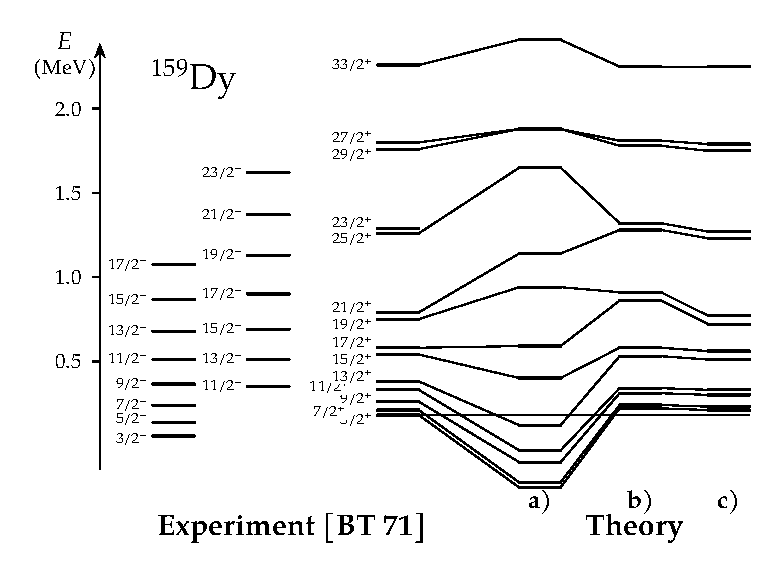
\includegraphics[width=0.75\textwidth]{pictures/3_11}
\par\end{centering}
\caption{\label{fig:3.11}$^{159}\text{Dy}$ 核中的三条转动带。$3/2^{-}$ 与 $11/2^{-}$
带是强耦合的（$\Delta I=1$）。带头为 $I=5/2$ 的正宇称带受到强烈微扰，如正文中所讨论。将其与三种理论计算进行了比较：(a)
无衰减 $\rho$ 的粒子加转子拟合；(b) 引入衰减因子 $\rho=0.5$ 的粒子加转子拟合；(c) 根据式 (3.56)
自洽确定的衰减。（引自 \cite{Ri77}。）}
\end{figure}

为了描述这些能带，人们通常在强耦合基 \ref{eq:3.25} 下对角化 Hamilton 量 \ref{eq:3.10}。单（准）粒子能量取自
Nilsson 模型，而形变 $\beta$（以及配对能隙 $\Delta$，参见第 6 章）等参数则用于拟合能谱。计算表明，只有引入一个削弱
Coriolis 相互作用的额外参数 $\rho$——即\emph{衰减因子}（attenuation factor），也就是用
$\rho\cdot H_{\text{cor}}$ 代替 $H_{\text{cor}}$ \cite{HRH70,LRB72,HK77}，才能够重现实验能谱。原始的
Coriolis 力被证实过于强烈，必须乘以因子 $\rho\sim0.4-0.8$ 予以缩减。通过这种唯象的衰减并合理选取模型的其他参数，我们能够成功重现这些畸变带，并发现对于低
$I$ 值（即较弱的 Coriolis 相互作用），体系处于 $\Delta I=1$ 的强耦合极限；然而对于更高的 $I$
值，Coriolis 力变得更强，并将具有高 $j$ 值的奇粒子平行于转动轴顺排。对于 $I\gtrsim j$ 的 $I$
值，体系具有转动顺排运动，即强烈的 $K$ 混合，能带分裂为 $(I-j)$ 为偶数时具有最大顺排 $\alpha=j$ 的优选态，以及
$(I-j)$ 为奇数时顺排较小的非优选态（$\alpha=j-1$）。对于由 $R=I-\alpha$ 给出的相同的核心角动量
$R$ 值，这两条带几乎是简并的（参见\ref{fig:3.11}）。

人们做出了若干尝试，在线性响应理论框架下将衰减因子解释为一种有效电荷 \cite{BPC72,HK75}。事实证明，这一问题与反冲项
\ref{eq:3.22} 的妥善处理紧密相关。认为反冲项已在拟合带头能量时被计入的观点并不成立，因为在单粒子情形下反冲项正比于
$\boldsymbol{j}^{2}-K^{2}$，具有强烈的 $K$ 依赖性并移动各带头的位置 \cite{ORG75}。

为了定性理解反冲项的作用，我们限制在仅有一个粒子的情形，并将粒子加转子 Hamilton 量 {[}\ref{eq:3.20} 等{]}
改写为如下形式 \cite{Kr79}：

\begin{equation}
H=H_{\text{intr}}+\frac{1}{2\mathcal{J}}\left(I(I+1)-\boldsymbol{j}^{2}\right)+H_{\text{cor}}'\label{eq:3.50}
\end{equation}
其中新的 Coriolis 项为

\begin{equation}
H_{\text{cor}}'=-\frac{1}{\mathcal{J}}(\boldsymbol{I}-\boldsymbol{j})\cdot\boldsymbol{j}_{\perp}=-\frac{1}{\mathcal{J}}\boldsymbol{R}\cdot\boldsymbol{j}=-\boldsymbol{\omega}\cdot\boldsymbol{j}\label{eq:3.51}
\end{equation}
其中集体角速度由下式给出：

\begin{equation}
\boldsymbol{\omega}=-\boldsymbol{R}/\mathcal{J}\label{eq:3.52}
\end{equation}
\ref{eq:3.51} 中的 Coriolis 项 $H_{\text{cor}}'$ 相比于 $H_{\text{cor}}$
{[}\ref{eq:3.23}{]} 发生了衰减。为了看清这一点，我们进入奇粒子几乎完全顺排于集体转动 $\boldsymbol{R}$
的极限情形。此时我们有

\begin{equation}
\boldsymbol{R}\simeq\boldsymbol{I}_{\perp}\left(1-\frac{\alpha}{I}\right)\label{eq:3.53}
\end{equation}
并发现 $H_{\text{cor}}'$ 在这种情形下正比于 $H_{\text{cor}}$：

\begin{equation}
H_{\text{cor}}'=\left(1-\frac{\alpha}{I}\right)H_{\text{cor}}=\rho\cdot H_{\text{cor}}\label{eq:3.54}
\end{equation}
带有一个依赖于 $I$ 的衰减因子：

\begin{equation}
\rho=1-\frac{\alpha}{I}\label{eq:3.55}
\end{equation}
只有在极高的 $I$ 值下衰减才会消失。

到目前为止，关于反冲项影响的讨论仅局限于该算符的纯单粒子部分。实际上，它还包含一个两体相互作用项 $\boldsymbol{j}_{ik}\cdot\boldsymbol{j}_{lm}a^{\dagger}_{i}a^{\dagger}_{l}a_{m}a_{k}$，它产生了与核心粒子的相互作用。我们可以在平均场近似下处理该项
\cite{Ri77}，最终得到一个自洽衰减因子：

\begin{equation}
\rho=1-\frac{\langle j_{1}\rangle}{\sqrt{I(I+1)-\langle j^{2}_{3}\rangle}}\label{eq:3.56}
\end{equation}
在完全顺排的极限下，它过渡到\ref{eq:3.55} 的形式。我们还可以证明，这种近似等价于 cranking 模型（参见 3.4
节）。在自洽 cranking 模型框架下对奇 $A$ 核转动带的微观处理中（参见 7.7 节），Coriolis 相互作用的衰减被自动包含进来了
\cite{RMB74,RM74}。

\subsubsection{偶偶核中的回弯现象}

回弯现象（参见 3.2.4 节）已被 Stephens 和 Simon \cite{SS72a} 解释为 $1i_{13/2}$
壳层中两个中子的顺排。如果这两个中子不是绕 3 轴旋转，而是沿原子核的转动轴顺排，这便增加了额外的 $13/2+11/2=12$
个单位的角动量。因此，原子核可以通过添加单粒子角动量来降低其集体转动，同时增加其总角动量。

为了在数学上描述这一物理构想，Stephens 和 Simon 对角化了 Hamilton 量 \ref{eq:3.10}（包含
Coriolis 项的衰减），所选取的基底为未受微扰核心的 Slater 行列式

\[
|\Phi_{0}\rangle=|IMK=0\rangle
\]
以及两准粒子激发态（参见第 7 章）：

\begin{equation}
|\Phi_{K}\rangle=\beta^{\dagger}_{K_{1}}\beta^{\dagger}_{K_{2}}|IMK=K_{1}+K_{2}\rangle\label{eq:3.57}
\end{equation}
其中 $\beta^{\dagger}_{K}$ 是 $1i_{13/2}$ 壳层中处于 $\Omega=K$ 态的准粒子产生算符。

对于低 $I$ 值，晕态主要由纯转子的零准粒子态 $|\Phi_{0}\rangle$ 给出。激发带是两准粒子带。对于更高的 $I$
值，粒子将其角动量沿转动轴顺排，其中一个顺排至 $\alpha=j=13/2$，第二个顺排至 $\alpha=j-1=11/2$。这样我们发现态
$\Phi_{0}$ 与 $\Phi_{K}$（$K=0,1,\dots$）发生混合，并在完全顺排的极限下达到如下形式的两准粒子态{[}参见\ref{eq:3.44}{]}：

\begin{equation}
|\Phi\rangle_{\text{al}}=\sum_{K_{1}K_{2}}d^{j}_{K_{1}j}\left(-\frac{\pi}{2}\right)d^{j}_{K_{2}j-1}\left(-\frac{\pi}{2}\right)\beta^{\dagger}_{K_{1}}\beta^{\dagger}_{K_{2}}|IMK_{1}+K_{2}\rangle\label{eq:3.58}
\end{equation}
它可以示意性地写作 $\tilde{\beta}^{\dagger}_{j}\tilde{\beta}^{\dagger}_{j-1}|\Phi_{0}\rangle$，其中
$\tilde{\beta}^{\dagger}_{\alpha}$ 是沿 1 轴量子化的准粒子算符。

Stephens 和 Simon \cite{SS72a} 利用这一方法相当好地重现了实验上的回弯能谱。然而，由于他们未曾计入由
Coriolis 反配对效应引起的对关联的渐进变化，他们无法获得低自旋值下对 $I(I+1)$ 定律的偏离。

尽管该模型适当地描述了两个顺排粒子的重要效应，但它无法使我们断定是否存在任何其他机制可能成为观测到的回弯现象的起源。为了判决它究竟是由形状变化、向正常流体态的相变还是顺排过程所引起的，人们必须开展计入所有这些自由度的微观计算。此类研究已经展开（参见
7.7 节）。它们表明两个粒子的转动顺排是最主要的效应。在所有含有高 $j$ 壳层的核中都可以发现这一过程。至于它们是否产生回弯，最终取决于相互作用矩阵元的强度（能级交叉处两能带之间的相互作用）：只有在弱矩阵元的情形下，我们才会观测到突变跃迁，即回弯现象\footnote{Bengtsson 等人 \cite{BHM78} 发现该相互作用作为化学势 $\lambda$ 的函数呈现振荡行为。对该事实的解释参见
\cite{FPS80} 及其所列参考文献。}。

\subsection{三轴粒子加转子模型}

我们在 1.5.3 节中已经看到，Davydov 等人 \cite{DF58} 利用三轴转子来解释某些过渡核中低激发的 $2^{+}$
态。通过将一个外层粒子耦合到三轴转子上，该模型也可以推广到奇 $A$ 核 \cite{Pa61,HS62,PR62,PS65,MSD74,Me75,FT75,TF75,Le76,DF77,LLR78}。它已被应用于外层粒子处于高
$j$ 壳层的情形，并在描述许多过渡核的能级与衰变纲图方面显示出极强的威力\footnote{关于三轴转子模型向多粒子组态的推广，参见 \cite{TNV77,YTF77,TYF77,YTF78}。}。然而目前尚缺乏微观基础。利用微观理论计算这些质量区域的静态能量势能面，并未展现出三轴形变处存在深极小值来为此简易物理图像提供依据。事实上，还存在基于振动图像的其他模型
\cite{AP76,PVD77,YNN76}，它们同样能够重现这些能谱。目前尚不清楚过渡核的这两种物理图像之间是否存在内在联系。

在接下来的讨论中，我们限制在一个高 $j$ 壳层（例如 $1h_{11/2}$）中的单个外层粒子耦合到三轴转子的情形。在此情形下，Hamilton
量具有如下形式 \cite{MSD74}：

\begin{equation}
h=\sum^{3}_{i=1}\frac{R^{2}_{i}}{2\mathcal{J}_{i}}+h_{0}+kr^{2}\beta\left\{ \cos\gamma\,Y_{20}+\sin\gamma\,\frac{1}{\sqrt{2}}\left(Y_{22}+Y_{2-2}\right)\right\} \label{eq:3.59}
\end{equation}
转动惯量 $\mathcal{J}_{i}$ 对 $\beta,\gamma$ 的依赖关系取自无旋流模型{[}式 (1.48){]}，仅对其整体常数进行调节。常数
$k$ 由 Nilsson 方案中 $j$ 壳层的分裂给出。$h_{0}$ 是球形谐振子 Hamilton 量。通常也计入具有常能隙
$\Delta$ 的单粒子配对场。

\ref{fig:3.12} 给出了在典型形变 $\beta=54A^{-2/3}$ 下，Hamilton 量 \ref{eq:3.59}
的能谱作为 $\gamma$ 的函数。在长椭球一侧（$\gamma=0^{\circ}$）和扁椭球一侧（$\gamma=60^{\circ}$），我们再次看到与\ref{fig:3.10}
中相同的能谱。然而，这两个极限现在是通过 $(\beta,\gamma)$ 平面内一条保持形变 $\beta$ 恒定的圆弧（图
1.4）相连接的。我们不再穿过 $\beta=0$ 处的弱耦合极限。在这两端，能谱对三轴参数 $\gamma$ 的依赖性并不十分剧烈。从强耦合方案到解耦方案的实质性转变发生在
$\gamma=30^{\circ}$ 附近的相对狭窄的 $\gamma$ 区域内。在弱形变过渡核中有许多能谱能够通过 $20^{\circ}$
到 $40^{\circ}$ 之间的 $\gamma$ 值极好地重现。通过在可变转动惯量（VMI）模型类型的计算中计入转动惯量的变化，这种一致性还可以得到进一步改善
\cite{FT75}。

\begin{figure}[H]
\begin{centering}
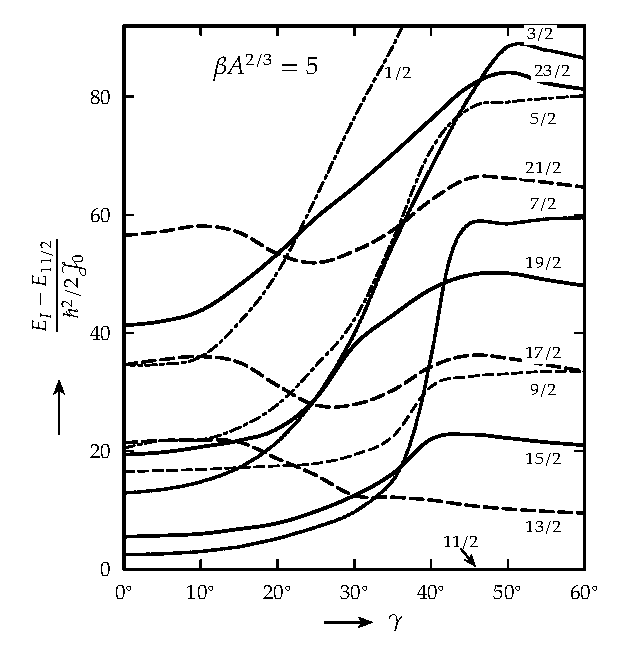
\includegraphics[width=0.75\textwidth]{pictures/3_12}
\par\end{centering}
\caption{\label{fig:3.12}一个 $j=11/2$ 粒子与非对称转子耦合的能谱，展示所有 $I\leqslant23/2$
的晕能级作为 $\gamma$ 的函数。（引自 \cite{MSD74}。）}
\end{figure}

一个奇高 $j$ 粒子与旋转三轴核心耦合系统的动力学行为由三种物理效应决定（参见 \cite{Me75}）：
\begin{enumerate}
\item[(i)] 核心倾向于绕具有最大转动惯量的轴旋转，以极小化转动能。
\item[(ii)] 在形变势阱中运动的粒子倾向于与核心取得最大的质量重叠，因为在此情形下其势能最小。
\item[(iii)] Coriolis 相互作用力图使粒子的角动量 $\boldsymbol{j}$ 与核心的角动量 $\boldsymbol{R}$
彼此顺排。
\end{enumerate}
对于高 $j$ 值，只要我们在 $j$ 壳层中仅有一个粒子，顺排效应便占据主导地位。由于顺排粒子的密度分布是以 $\boldsymbol{j}$
为对称轴的扁椭球，若核心为扁椭球（$\gamma=60^{\circ}$），对应于以 2 轴为对称轴，则条件 (ii) 得到最佳满足。然而在此情形下
$\mathcal{J}_{2}=0$，条件 (i) 受到了破坏。因此 $\boldsymbol{R}$ 将垂直于 2 轴，我们不再具有顺排。在三轴情形下，$\mathcal{J}_{2}$
不再为零，条件 (i)、(ii) 与 (iii) 可以全部同时得到满足。此时出现 $\boldsymbol{j}$ 与 $\boldsymbol{I}$
沿着 2 轴的顺排。事实上计算表明，奇粒子倾向于沿核心的 2 轴顺排。该轴起到近似对称轴的作用，其含义在于近似量子数 $K$ 与
$\Omega$（分别代表 $\boldsymbol{I}$ 与 $\boldsymbol{j}$ 在 2 轴上的投影）对于能级分类是有意义的。其结果是产生具有三轴转子特征的全新能级方案。

正如 Stephens 的转动顺排耦合方案那样，晕能级由 $\Omega=j$ 以及 $K=j,j+2,j+4$ 给出。对于这些能级，$\boldsymbol{I}$、$\boldsymbol{j}$、$\boldsymbol{R}$
以及 2 轴彼此平行。它们位于具有 $\Delta I=2$ 的通常抛物线上（参见\ref{fig:3.13}）。在轴对称情形下，顺排的方向在
1-2 平面内是任意的（通常选取 1 轴）；与之相反，非对称情形没有这种对称性，顺排明显青睐于 2 轴。这导致的推论是，在每一个晕能级上都存在自旋次序为
$\Delta I=1$ 的转动带。事实上，实验上已经观测到了这类能级 \cite{ABR75}。

\begin{figure}[H]
\begin{centering}
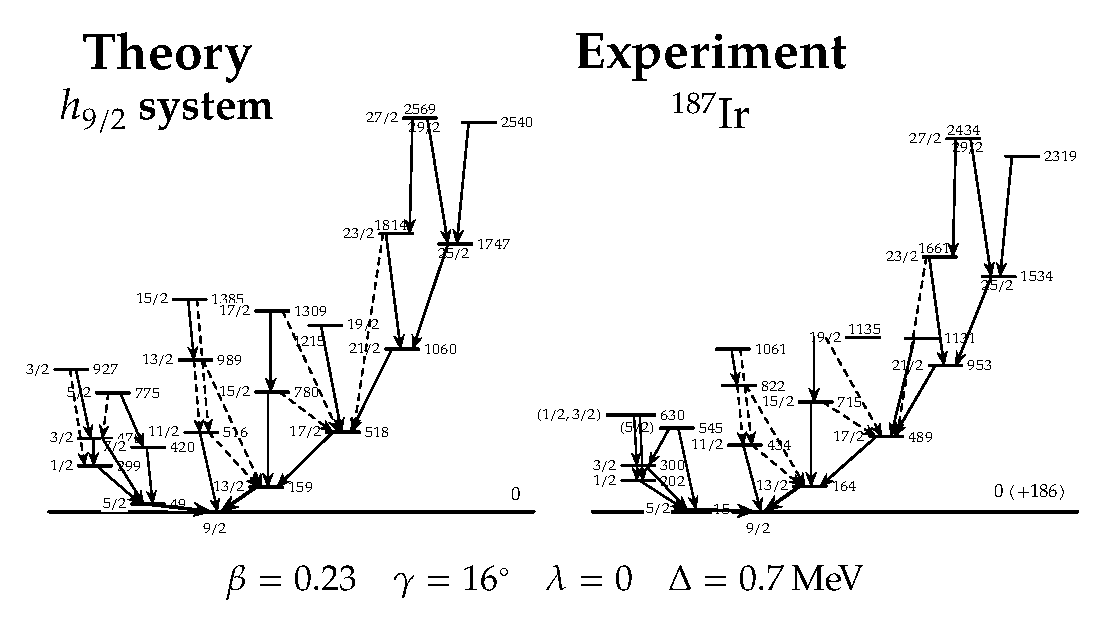
\includegraphics[width=0.75\textwidth]{pictures/3_13}
\par\end{centering}
\caption{\label{fig:3.13}$^{187}\text{Ir}$ 中负宇称态的 $1h_{9/2}$ 家族。（引自 \cite{Me75}。）}
\end{figure}


\subsection{电磁性质}

根据将系统划分为价粒子与核心的做法，电磁多极算符也相应地包含两部分贡献：

\begin{equation}
Q_{\lambda\mu}=Q^{(c)}_{\lambda\mu}+Q^{(p)}_{\lambda\mu}\label{eq:3.60}
\end{equation}
核心部分由式 (1.35) 给出，而 $Q^{(p)}$ 在式 (B.23)、(B.24) 中定义，其中对 $i$ 的求和仅限于价粒子的数目。

在接下来的讨论中，我们将限制在没有对关联的轴对称情形。随后将这些公式推广到更复杂的情形是相对简单的。

转子的磁偶极矩由式 (1.36) 给出为 $\boldsymbol{\mu}=g_{R}\mu_{N}\boldsymbol{R}$。因此对于
$M1$ 算符我们获得：

\begin{equation}
\boldsymbol{M}_{1}=\sqrt{\frac{3}{4\pi}}\mu_{N}g_{R}(\boldsymbol{I}-\boldsymbol{j})+\boldsymbol{M}^{(p)}_{1}\label{eq:3.61}
\end{equation}
磁偶极矩在式 (B.31) 中定义。利用\ref{eq:3.25} 的波函数并应用投影定理 (2.66)，对于 $K\neq1/2$
我们得到：

\begin{equation}
\mu=\sqrt{\frac{4\pi}{3}}\langle\Psi^{I}_{IK}|M_{1z}|\Psi^{I}_{IK}\rangle=\mu_{N}\left\{ g_{R}\frac{I(I+1)-K^{2}}{I+1}+g_{K}\frac{K^{2}}{I+1}\right\} \label{eq:3.62}
\end{equation}
其中我们以如下方式引入了回旋磁比 $g_{K}$：

\begin{align}
g_{K}\cdot K & =\frac{1}{\mu_{N}}\sqrt{\frac{4\pi}{3}}\langle\Phi_{K}|M^{(p)}_{13}|\Phi_{K}\rangle\nonumber \\
 & =\langle\Phi_{K}|g_{s}s_{3}+g_{l}l_{3}|\Phi_{K}\rangle\nonumber \\
 & =g_{l}K+(g_{s}-g_{l})\langle\Phi_{K}|s_{3}|\Phi_{K}\rangle\label{eq:3.63}
\end{align}
矩阵元 $\langle\Phi_{K}|s_{3}|\Phi_{K}\rangle$ 可以利用 Nilsson 波函数算出。对于
$K=1/2$，磁矩获得一个包含\ref{eq:3.30} 中解耦因子 $a$ 的额外贡献。

利用\ref{eq:3.62} 获得的磁矩已在广泛的原子核范围进行了计算 \cite[第 653 页]{MN59,NN65}，人们发现与实验数据的一致性通常质子优于中子。详细的研究表明，人们同样需要对
$g_{s}$ 引入极化电荷：$g^{\text{eff}}_{s}\simeq0.7g^{\text{free}}_{s}$（参见
\cite[第 302 页起]{BM75}）。

类似地，我们可以计算 $M1$ 跃迁的约化矩阵元。算符 $\boldsymbol{I}$ 不引起任何跃迁。对于其余部分我们利用式
(1.70)，对于 $K\neq1/2$ 且 $I_{i}\neq I_{f}$ 得到：

\begin{equation}
B(M1,I_{i}\to I_{f})=\frac{1}{2I_{i}+1}|\langle\Psi^{I_{f}}_{K}\|\boldsymbol{M}_{1}\|\Psi^{I_{i}}_{K}\rangle|^{2}=\frac{3}{4\pi}\mu^{2}_{N}(g_{K}-g_{R})^{2}K^{2}|C^{I_{i}\ 1\ I_{f}}_{K\ 0\ K}|^{2}\label{eq:3.64}
\end{equation}
这些 $M1$ 跃迁仅可能存在于奇 $A$ 核的转动带中。计算结果与实验符合得相当好 \cite{SBP67}。

再次利用式 (1.70)，我们还可以导出电四极跃迁的 $B(E2)$ 值。对于相同 $K$ 值的态之间的跃迁，由于核心具有巨大的
$Q_{0}$ 值，核心贡献远大于粒子贡献。因此粒子贡献可以忽略，我们得到：

\begin{equation}
B(E2,I_{i}\to I_{f})=Q^{2}_{0}\frac{5}{16\pi}|C^{I_{i}\ 2\ I_{f}}_{K\ 0\ K}|^{2}\label{eq:3.65}
\end{equation}
该方程用于确定出现在 $Q_{0}$ 中的形变实验值。在 2.8.6 节中我们看到它们与理论确定的形变相符合。因此，粒子加转子模型对于具有相同
$K$ 值的跃迁给出了适宜的 $E2$ 跃迁几率。

对于具有不同 $K$ 值的跃迁，集体部分消失。此类跃迁实际上非常微弱（$K$ 禁戒，$K$-forbidden），因为单粒子部分仅包含内禀系中
$r^{2}Y_{20}$ 的单粒子矩阵元。我们在 2.7.2 节中已经看到，它们与集体跃迁值相比是极其微小的。另一方面，纯单粒子模型无法解释球形核中的有效电荷（参见
2.7.2 节）。同样的困难在此再次出现。关于详细讨论，请参阅 Löbner 和 Malmskog 的论文 \cite{LM66}，其中包含了大量实验数据以及改进简易
Nilsson 估计的可能途径。

最后我们必须提及，上述考虑仅适用于纯 $K$ 带。对于 $K$ 混合带中的跃迁几率与电磁矩（例如转动顺排带或非对称转子中的能带），我们必须计入混合系数。

\section{Cranking 模型\protect\footnote{在本章中，我们仅讨论用于转动的 cranking 理论。然而，正如在 12.3.7 节中所讨论的，我们也可以将类似理论应用于一般的集体运动。}}

我们在上一节中已经看到，形变势阱中的粒子运动如何能够与刚性转子的概念联系起来。该模型在描述转动核乃至过渡核的能级结构方面取得了巨大的成功。然而，它并不存在直接了当的微观推导；特别是在该模型中人们无法微观计算惯性参数。

另一方面，几乎所有关于原子核转动的完全微观的理论，都以某种方式基于或关联于由 Inglis \cite{In54,In56} 以半经典方式引入的\emph{推引模型}（cranking
model）。正如我们在 11.4 节中将要看到的，至少在强形变且 $K$ 掺杂不太强烈（$K\ll I$）的极限下，它可以完全从量子力学推导出来。

Cranking 模型具有以下显著优点：
\begin{enumerate}
\item[(i)] 原则上，它提供了旋转原子核的完全微观描述。该模型没有引入冗余变量，因此我们能够在模型内部微观地计算转动惯性参数，并深入洞悉转动运动的动力学本质。
\item[(ii)] 它将集体角动量描述为各单粒子角动量之和。因此，集体转动、单粒子转动以及它们之间的所有过渡（例如解耦过程），都在相同的基准上得到了统一的处理。
\item[(iii)] 对于非常高的角动量，经典论据完全适用，该模型是完全正确的（即使在这一极限下量子力学推导不再有效 \cite{BMR70}）。
\end{enumerate}
该模型的局限性在于：
\begin{enumerate}
\item[(i)] 正如我们将看到的，它本质上是一个非线性理论。只有在小角动量极限下，人们才能利用微扰论将其线性化（得到转动惯量的 cranking
公式）。在一般情形下计算因此变得复杂，特别是在具有多个解的情况下。
\item[(ii)] 由此得到的波函数不是角动量算符的本征态。因此，先验地如何计算例如电磁跃迁几率并不清晰。事实上，我们在 11.4 节中将看到，cranking
模型的波函数在某种意义上仅是内部波函数，必须使用投影技术才能获得实验室坐标系中的波函数。
\end{enumerate}
在下文中，我们将给出通常的半经典推导（例如参见 \cite{Vi57b,So73}），并结合纯单粒子 Hamilton 量讨论 cranking
模型。随后几节中的许多论据，也可以直接推广到一般的两体 Hamilton 量中（参见 7.7 节）。

\subsection{Cranking 模型的半经典推导}

Cranking 模型的基本思想基于如下经典假设：如果引入一个以恒定角速度 $\boldsymbol{\omega}$ 绕空间固定轴转动的参考系，若角频率选取适当，核子在转动参考系中的运动将相当简单；特别是，核子可以被视为独立粒子，运动于一个随坐标系共同转动的平均势阱之中。

在 11.4 节中，我们将看到如何利用投影技术从量子力学推导出这一物理图像的结论。然而目前，出于其直观性，我们仍希望保留经典描述。同时，我们暂不考虑任何剩余相互作用。因此，我们假设一个具有固定形状、在空间中转动的单粒子势
$V$，相应地我们必须考虑含时的单粒子 Hamilton 量：

\begin{equation}
h(t)=\frac{\boldsymbol{p}^{2}}{2m}+V(\boldsymbol{r},t)\label{eq:3.66}
\end{equation}
以及对应的 Schrödinger 方程：

\begin{equation}
h(t)\psi(t)=\mathrm{i}\hbar\frac{\partial}{\partial t}\psi(t)\label{eq:3.67}
\end{equation}
引入相对于转动轴 $\boldsymbol{\omega}$ 的球坐标 $r,\theta,\varphi$，我们可以将 $V(t)$
的时间依赖性表示为如下形式。若 $V(\boldsymbol{r},0)$ 是 $t=0$ 时的势，则在时刻 $t$ 有：

\begin{equation}
V(\boldsymbol{r},t)=V(r,\theta,\varphi-\omega t,0)\label{eq:3.68}
\end{equation}
我们再次认识到，$V$ 仅当它依赖于 $\varphi$ 时才显含时间。换言之，$V$ 不应当绕转动轴具有轴对称性，因为对于量子力学系统，绕对称轴不可能存在集体转动（参见
1.5.1 节）。由于\ref{eq:3.68} 中 $V(t)$ 具有非常简明的时间依赖性，存在一个消除此时间依赖性的幺正变换：

\begin{equation}
U=\mathrm{e}^{\mathrm{i}\boldsymbol{\omega}\cdot\boldsymbol{l}t/\hbar}\label{eq:3.69}
\end{equation}
其中 $\boldsymbol{\omega}\cdot\boldsymbol{l}=(\hbar/\mathrm{i})\omega\,\partial/\partial\varphi$。$U$
产生了绕转动轴 $\boldsymbol{\omega}$ 转动角度 $\omega t$ 的操作。

我们发现含时算符满足

\begin{equation}
Uh(t)U^{-1}=h(0)\label{eq:3.70}
\end{equation}
并定义变换后的波函数：

\begin{equation}
\tilde{\psi}=U\psi\label{eq:3.71}
\end{equation}
满足

\begin{equation}
\mathrm{i}\hbar\dot{\tilde{\psi}}=\mathrm{i}\hbar U\dot{\psi}+\mathrm{i}\hbar\dot{U}\psi=(h(0)-\boldsymbol{\omega}\cdot\boldsymbol{l})\tilde{\psi}\label{eq:3.72}
\end{equation}
\ref{eq:3.72} 是一个含有显含时间无关的有效 Hamilton 量 $h_{\omega}$ 的含时 Schrödinger
方程。因此它可以按标准方法化为一个本征值问题求解：

\begin{equation}
h_{\omega}\tilde{\psi}=(h(0)-\boldsymbol{\omega}\cdot\boldsymbol{l})\tilde{\psi}=\epsilon_{\omega}'\tilde{\psi}\label{eq:3.73}
\end{equation}
其中 $\epsilon_{\omega}'$ 是有效 Hamilton 量的本征值（又称 Routhian 本征值）。为了获得原始
Hamilton 量的能量，我们必须计算：

\begin{equation}
E_{k}=\langle\psi|h(t)|\psi\rangle=\langle\tilde{\psi}|h(0)|\tilde{\psi}\rangle=\epsilon_{k}'+\boldsymbol{\omega}\cdot\langle\tilde{\psi}|\boldsymbol{l}|\tilde{\psi}\rangle\label{eq:3.74}
\end{equation}
项 $\boldsymbol{\omega}\cdot\boldsymbol{l}$ 通常被称为 Coriolis 项。

我们现在求解了转动势中的含时 Schrödinger 方程，并发现我们必须对角化一个显含时间无关的有效 Hamilton 量。我们想强调的是，我们并非先验地推导从转动坐标系所看到的
Hamilton 量，因为我们仅变换了坐标而未变换动量。事实上，在纯平动运动的情形下，我们会得到类似的结果{[}$h_{v}=h(0)-\boldsymbol{v}\cdot\boldsymbol{p}${]}，但由
Galilei 不变性我们要求从运动参考系看到的 Hamilton 量与静止参考系相同。尽管如此，事实表明在转动的特殊情况下，\ref{eq:3.73}
中的 $h_{\omega}$ 与转动系统中所看到的 Hamilton 量是完全恒等的 \cite[第 69 页]{Va56,Br64}。从项
$\boldsymbol{\omega}\cdot\boldsymbol{l}$ 中，我们可以同时导出 Coriolis 力与离心力。

对于具有自旋的系统，产生转动的算符为 $\boldsymbol{j}=\boldsymbol{l}+\boldsymbol{s}$。转动轴的取向通常选取为平行于
$x$ 轴，因为人们理解转动轴垂直于对称轴（在 $\omega=0$ 时对称轴为 $z$ 轴）。对于更高的角动量，人们也研究非对称单粒子势。尽管如此，我们仍要求
$\boldsymbol{\omega}$ 平行于势的一个主轴。因此，cranking 模型的多体 Hamilton 量由下式给出（其中
$J_{x}=\sum^{A}_{i=1}j^{(i)}_{x}$）：

\begin{equation}
H_{\omega}=H-\omega J_{x}=\sum^{A}_{i=1}h^{(i)}_{\omega}\label{eq:3.75}
\end{equation}
其中 $H$ 是形变单粒子 Hamilton 量之和。

在 cranking 模型中，我们现在必须对角化 $H_{\omega}$，所得的基态波函数 $\Phi_{\omega}$ 是一个
Slater 行列式。正如在普通壳模型（$\omega=0$）中一样，出现了一个问题：应当如何填充分配单粒子势中的能级，以获得任意给定角动量下的最低能量状态（晕能级）？这一问题的答案（在
11.4 节中给出）是，我们必须极小化能量 $E'=\langle\Phi|H-\omega J_{x}|\Phi\rangle$，也就是说，我们必须在转动参考系中按通常的方式从低到高填充有效能级。

对于实验室坐标系中的能量，由\ref{eq:3.74} 我们得到：

\begin{equation}
E(\omega)=\langle\Phi_{\omega}|H|\Phi_{\omega}\rangle=\langle\Phi_{\omega}|H_{\omega}|\Phi_{\omega}\rangle+\omega\langle\Phi_{\omega}|J_{x}|\Phi_{\omega}\rangle\label{eq:3.76}
\end{equation}
由于 $E(\omega)$ 不能依赖于 $\omega$ 的符号，人们发现：

\begin{equation}
E(\omega)=E(0)+\frac{1}{2}\mathcal{J}_{1}\omega^{2}+\dots\label{eq:3.77}
\end{equation}
并且，由于在 $\omega=0$ 时 $\langle\Phi_{0}|J_{x}|\Phi_{0}\rangle=0$，

\begin{equation}
J(\omega)=\langle\Phi_{\omega}|J_{x}|\Phi_{\omega}\rangle=\mathcal{J}_{2}\omega+\dots\label{eq:3.78}
\end{equation}
利用 $E'(\omega)$ 是 $H_{\omega}$ 的最低本征值这一事实，我们可以证明常数 $\mathcal{J}_{1}$
与 $\mathcal{J}_{2}$ 是相等的 \cite{Sch61}：

\begin{equation}
\mathcal{J}_{1}=\mathcal{J}_{2}\label{eq:3.79}
\end{equation}
根据 Ritz 变分原理，我们获得 $\Phi_{\omega}$ 作为如下方程的解：

\begin{equation}
\delta\langle\Phi|H-\omega J_{x}|\Phi\rangle=0\label{eq:3.80}
\end{equation}
其中 $|\Phi\rangle$ 是所有可能 Slater 行列式集合中的任意一员。如果我们将 $|\Phi\rangle$
限制在子集 $\{\Phi_{\omega'}\}$ 中（其中 $\Phi_{\omega'}$ 是 $H-\omega'J_{x}$
的本征函数，$\omega'$ 遍历所有实数），该条件同样满足。于是由\ref{eq:3.80} 得到：

\begin{equation}
\left.\frac{\mathrm{d}}{\mathrm{d}\omega'}\langle\Phi_{\omega'}|H|\Phi_{\omega'}\rangle\right|_{\omega'=\omega}-\omega\left.\frac{\mathrm{d}}{\mathrm{d}\omega'}\langle\Phi_{\omega'}|J_{x}|\Phi_{\omega'}\rangle\right|_{\omega'=\omega}=0\label{eq:3.81}
\end{equation}
或者

\[
\mathcal{J}_{1}=\left.\frac{1}{\omega}\frac{\mathrm{d}}{\mathrm{d}\omega}E(\omega)\right|_{\omega=0}=\left.\frac{\mathrm{d}}{\mathrm{d}\omega}J(\omega)\right|_{\omega=0}=\mathcal{J}_{2}
\]
由\ref{eq:3.80} 我们还可以导出正则关系：

\begin{equation}
\omega=\frac{\mathrm{d}E}{\mathrm{d}J}\label{eq:3.82}
\end{equation}
为了与实验进行比较，我们必须确定角速度的值。Inglis \cite{In54} 建议至少在半经典意义上通过要求

\begin{equation}
J=\langle\Phi_{\omega}|J_{x}|\Phi_{\omega}\rangle=\sqrt{I(I+1)}\label{eq:3.83}
\end{equation}
来包含零点量子涨落。在一阶近似下我们得到

\begin{equation}
\omega=\frac{\sqrt{I(I+1)}}{\mathcal{J}_{1}}\label{eq:3.84}
\end{equation}
并由\ref{eq:3.77} 得到：

\begin{equation}
E(I)=E(0)+\frac{1}{2\mathcal{J}_{1}}I(I+1)\label{eq:3.85}
\end{equation}
对于更高的 $\omega$ 值，将出现对该 $I(I+1)$ 定律的偏离。一般而言，转动惯量定义为

\begin{equation}
\mathcal{J}=\frac{J}{\omega}\label{eq:3.86}
\end{equation}
到目前为止，我们仅研究了完全独立的粒子运动，这里的含义是我们甚至忽略了转动对平均场本身的反作用影响。在 7.7 节中我们将展示如何将该效应自洽地予以考虑。

\subsection{Cranking 公式}

在纯 $I(I+1)$ 能谱的情形下，我们只需计算一个常数，即转动惯量。它已经被 $2^{+}$ 态所完全确定，因此对于如此小的
$I$ 值应用微扰论显得十分有意义。

我们从形变势阱中被填充至 Fermi 面的未微扰系统出发。Fermi 面以下的能级被称为空穴态（指标 $i,l,\dots$）；Fermi
面以上的能级被称为粒子态（指标 $m,m',\dots$）。壳模型基底由基态 $|\Phi_{0}\rangle$、粒子-空穴态（ph
态）$|mi\rangle=a^{\dagger}_{m}a_{i}|\Phi_{0}\rangle$、2p-2h 态等构成。微扰
$\omega J_{x}$ 是一个单体算符，因此一次只能激发一个 ph 对。因此，对于一阶微扰波函数我们得到：

\begin{equation}
|\Phi\rangle=|\Phi_{0}\rangle+\omega\sum_{mi}\frac{\langle mi|J_{x}|\Phi_{0}\rangle}{\epsilon_{m}-\epsilon_{i}}a^{\dagger}_{m}a_{i}|\Phi_{0}\rangle\label{eq:3.87}
\end{equation}
其中 $\epsilon_{i}$ 与 $\epsilon_{m}$ 是 Hamilton 量 $H$ 的单粒子能量。至 $\omega$
的一阶，$J_{x}$ 的期望值为

\begin{equation}
J=\langle\Phi|J_{x}|\Phi\rangle=2\omega\sum_{mi}\frac{|\langle mi|J_{x}|\Phi_{0}\rangle|^{2}}{\epsilon_{m}-\epsilon_{i}}\label{eq:3.88}
\end{equation}
结合\ref{eq:3.78}，这给出了转动惯量\footnote{在分子物理学中，Wick \cite{Wi48} 曾推导出类似的公式。}：

\begin{equation}
\mathcal{J}_{\text{Inglis}}=2\sum_{mi}\frac{|\langle mi|J_{x}|\Phi_{0}\rangle|^{2}}{\epsilon_{m}-\epsilon_{i}}\label{eq:3.89}
\end{equation}
这就是著名的 Inglis 转动惯量公式 \cite{In54,BM55}。

由该公式算出的转动惯量通常非常接近刚体转动惯量的值{[}式 (1.49){]}。事实上，我们在 3.4.3 节中将看到，在纯各向异性谐振子势的情形下这甚至是一个严格的结果。Lüders
\cite{Lu60} 证明，对于任何独立粒子模型在大粒子数极限下均成立此结论（亦参见 \cite{AB59,Ro59,SB64,Da75,KG78}）。

我们可以定性地理解这一结果：只要我们认识到形变静态势中基态的速度分布几乎是各向同性的（参见 13.3 节），并且在转动系统中这一事实并未因
Coriolis 力或离心力而改变（参见 \cite{BJ76b}）。此时在内禀系中没有净流动，而在实验室参考系中我们观测到刚体转动的速度分布。

正如我们在 1.5.1 节中所见，实验上的转动惯量比它们的刚体值小 2 到 3 倍。Bohr 和 Mottelson \cite{BM55,Mo56}
早就指出，剩余两体相互作用会大幅降低这些数值。在这方面最重要的影响是对关联型的相互作用。由于在单粒子描述中它们可以在 BCS 形式体系内非常方便地予以包含（参见第
6 章），我们在此给出所谓的 Belyaev 公式 \cite{Be59,Be61} 的推导，它是包含了对关联的 Inglis \ref{eq:3.89}
的推广。（不熟悉该体系的读者请参阅第 6 章。）

在这种情形下，$|\text{BCS}\rangle$ 代表 BCS 基态 (6.31)，激发态由两准粒子态 $\alpha^{\dagger}_{k}\alpha^{\dagger}_{k'}|\text{BCS}\rangle$、四准粒子态等给出。与\ref{eq:3.87}
完全类似地，我们得到受微扰的波函数：

\begin{equation}
|\Phi\rangle=|\text{BCS}\rangle+\omega\sum_{k<k'}\frac{\langle\text{BCS}|J_{x}|kk'\rangle}{E_{k}+E_{k'}}\alpha^{\dagger}_{k}\alpha^{\dagger}_{k'}|\text{BCS}\rangle\label{eq:3.90}
\end{equation}
其中 $E_{k}+E_{k'}$ 是准粒子对 $k,k'$ 的激发能量。准粒子能量由下式给出：

\begin{equation}
E_{k}=\sqrt{(\epsilon_{k}-\lambda)^{2}+\Delta^{2}}\label{eq:3.91}
\end{equation}
仿照\ref{eq:3.88} 与 \ref{eq:3.89}，我们求得转动惯量：

\begin{equation}
\mathcal{J}_{\text{Belyaev}}=2\sum_{k<k'}\frac{|\langle\text{BCS}|J_{x}|kk'\rangle|^{2}}{E_{k}+E_{k'}}\label{eq:3.92}
\end{equation}
由式 (E.16)，我们求得 $J_{x}$ 的两准粒子矩阵元，并最终得到：

\begin{equation}
\mathcal{J}_{\text{Belyaev}}=2\sum_{k,k'>0}\frac{|\langle k|j_{x}|k'\rangle|^{2}}{E_{k}+E_{k'}}\left(u_{k}v_{k'}-u_{k'}v_{k}\right)^{2}\label{eq:3.93}
\end{equation}
与\ref{eq:3.89} 相比，该转动惯量公式确实给出了大幅降低的值。导致这一降低的有两个效应：
\begin{enumerate}
\item[(i)] 能量分母远大于\ref{eq:3.89} 中的粒子-空穴能量。参数 $\Delta$ {[}\ref{eq:3.91}{]}
对 Fermi 面附近的关键能级产生了至少 $2\Delta\sim2\,\text{MeV}$ 的能隙；
\item[(ii)] 因子 $(u_{k}v_{k'}-u_{k'}v_{k})^{2}$ 通常明显小于 1。
\end{enumerate}
BCS 理论中转动惯量相比于刚体值的降低，对应于原子核转动时部分核子的“超流滑移”（superfluid slippage）\cite{Mi59,Mi60}。

针对真实原子核的大规模数值计算 \cite{GR60b,NP61,MT75} 显示出与实验值极其显著的符合。正如我们在下一小节中将看到的，将
Inglis 或 Belyaev 公式应用于自洽波函数（即在对应于能量极小值的形变下计算出的波函数）是至关重要的。在大多数此类计算中，这是通过在实验观测到的形变下使用
Nilsson 波函数与能量、并采用实验确定的配对能隙 $\Delta$ 来实现的（亦参见 \cite{MN59}）。

这些计算给出的转动惯量大致落在（过小的）无旋流值与（过大的）刚体值之间，其巨大的成功给予我们极大的信心：将转动核视为形变超流多体系统的物理图像是完全正确的。

当然，我们还可以研究剩余相互作用对转动惯量的进一步影响。这可以在线性响应理论框架下进行（参见 8.5.3 节与 \cite{MSV72}）。在此类理论中，由
Coriolis 算符 $J_{x}$ 代表的外场可以激发核心的虚振动，这些振动反过来对转动惯量产生影响。存在两类此类振动：表面振荡（ph
振动，对应于拉伸效应），以及对关联中的振荡（pp 振动，参见 8.3.5 节）。此类计算的综合结果是，这两种效应大致相互抵消，我们得到的转动惯量数值（\ref{fig:3.14}）与
BCS 理论给出的结果基本相同。

\begin{figure}[H]
\begin{centering}
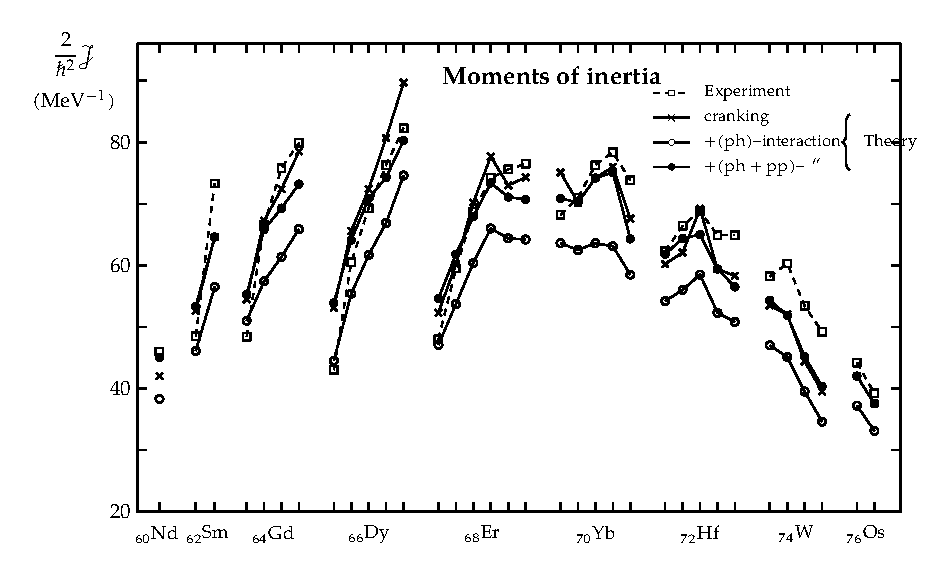
\includegraphics[width=0.75\textwidth]{pictures/3_14}
\par\end{centering}
\caption{\label{fig:3.14}稀土核中的转动惯量。方块表示实验值 \cite{NP61}；十字是由 Belyaev 公式 (3.93)
算得的结果。空心圆圈仅计入了拉伸效应（ph 相互作用）；除此之外，实心圆圈还计入了反配对效应（pp 相互作用）。（引自 \cite{MSV72}。）}
\end{figure}

我们现在已经讨论了应用微扰论计算 $J_{x}$ 的期望值（即转动惯量）。以类似的方式，我们还可以计算旋转核的其他性质，例如回旋磁比
$g_{R}$ 或第一 $2^{+}$ 态的磁矩。由于磁矩 $\mu$ 定义为 $M_{1z}$ 在态 $|I,M=I\rangle$
中的期望值{[}式 (B.31){]}，而 cranking 模型的波函数不是角动量的本征态，此时如何计算 $\mu$ 尚不明确。在
11.4 节中我们将看到必须应用投影技术。在最低阶近似下，我们获得一个非常简单的结果，它在 cranking 模型的半经典图像中极易理解：

\begin{equation}
\mu=\langle\Phi_{\omega}|M_{x}|\Phi_{\omega}\rangle\label{eq:3.94}
\end{equation}
因此我们可以通过下式定义回旋磁比 (1.37)：

\begin{equation}
\mu=g_{R}J=g_{R}\langle\Phi_{\omega}|J_{x}|\Phi_{\omega}\rangle\label{eq:3.95}
\end{equation}
由\ref{eq:3.90}，在一阶微扰论下我们得到：

\begin{equation}
g_{R}=\frac{1}{\mathcal{J}}\sum_{k,k'>0}\frac{\langle k|j_{x}|k'\rangle\langle k'|M_{x}|k\rangle+\text{c.c.}}{E_{k}+E_{k'}}\left(u_{k}v_{k'}-u_{k'}v_{k}\right)^{2}\label{eq:3.96}
\end{equation}
利用这些公式计算出的数值小于液滴模型的值 $g_{R}=Z/A$ {[}式 (1.37){]}，并与实验数据符合得相当好 \cite{MSV72}。

正如我们在 3.2 节中所见，当我们走向更高的角动量时，将出现对 $I(I+1)$ 定律的偏离。为了计算与这些偏离相联系的 $B$
与 $C$ 系数{[}式 (3.1){]}，人们使用了更高阶的微扰论，并计入了剩余相互作用的效应 \cite{Ma65,Ma67a,MR70}，其中最重要的效应是所谓的
Coriolis 反配对（CAP）效应，我们将在 7.7 节中对此进行讨论。正如我们将看到的，只有在自旋极高（$I>30$ 或 40）的态上，人们才能预期对关联彻底消失。

\subsection{转动各向异性谐振子}

我们在 2.8.3 节中已经看到，各向异性谐振子可以解析求解，并且它至少为形变核提供了一个定性模型。事实表明，它在转动参考系中同样可以解析求解（参见
\cite{Va56,Ze75,RBK75,GMZ78}），因为 $l_{x}=yp_{z}-zp_{y}$ 在坐标 $x,y,z$
和动量 $p_{x},p_{y},p_{z}$ 中是一个二次型。

我们可以暂且忽略自旋，因为势阱不依赖于自旋（Coriolis 算符中的项 $-\omega s_{x}$ 可以在自旋空间中独立对角化，仅产生一个对角贡献）。此时
Hamilton 量具有形式：

\begin{equation}
h_{\omega}=-\frac{\hbar^{2}}{2m}\nabla^{2}+\frac{1}{2}m\left(\omega^{2}_{x}x^{2}+\omega^{2}_{y}y^{2}+\omega^{2}_{z}z^{2}\right)-\omega\left(yp_{z}-zp_{y}\right)\label{eq:3.97}
\end{equation}
我们引入 $x,y,z$ 方向谐振子玻色子的产生和湮灭算符 $a_{x},a_{y},a_{z}$：

\begin{align}
x & =\left(\frac{\hbar}{2m\omega_{x}}\right)^{1/2}\left(a_{x}+a^{\dagger}_{x}\right),\quad p_{x}=\frac{\hbar}{\mathrm{i}}\left(\frac{m\omega_{x}}{2\hbar}\right)^{1/2}\left(a_{x}-a^{\dagger}_{x}\right)\nonumber \\
y & =\left(\frac{\hbar}{2m\omega_{y}}\right)^{1/2}\left(a_{y}+a^{\dagger}_{y}\right),\quad p_{y}=\frac{\hbar}{\mathrm{i}}\left(\frac{m\omega_{y}}{2\hbar}\right)^{1/2}\left(a_{y}-a^{\dagger}_{y}\right)\label{eq:3.98}\\
z & =\left(\frac{\hbar}{2m\omega_{z}}\right)^{1/2}\left(a_{z}+a^{\dagger}_{z}\right),\quad p_{z}=\frac{\hbar}{\mathrm{i}}\left(\frac{m\omega_{z}}{2\hbar}\right)^{1/2}\left(a_{z}-a^{\dagger}_{z}\right)\nonumber 
\end{align}
利用这些算符，$h_{\omega}$ 具有形式：

\begin{align}
h_{\omega} & =\hbar\omega_{x}\left(a^{\dagger}_{x}a_{x}+\frac{1}{2}\right)+\hbar\omega_{y}\left(a^{\dagger}_{y}a_{y}+\frac{1}{2}\right)+\hbar\omega_{z}\left(a^{\dagger}_{z}a_{z}+\frac{1}{2}\right)\nonumber \\
 & \quad+\frac{\hbar\omega}{2\sqrt{\omega_{y}\omega_{z}}}\left\{ (\omega_{y}-\omega_{z})\left(a^{\dagger}_{y}a^{\dagger}_{z}+a_{y}a_{z}\right)+(\omega_{y}+\omega_{z})\left(a^{\dagger}_{y}a_{z}+a^{\dagger}_{z}a_{y}\right)\right\} \label{eq:3.99}
\end{align}
\ref{eq:3.99} 中的 Coriolis 算符包含两部分贡献。第一部分产生或湮灭两个振子量子；因此它将主量子数为 $N$
与 $N\mp2$ 的壳层耦合起来\footnote{在微小形变极限下（$\omega_{y}\to\omega_{z}$）该项消失，因此常常被忽略 \cite{ALL76}。}。第二部分保持量子总数守恒，但将振子量子从
$y$ 方向转移到 $z$ 方向，反之亦然。

\subsubsection{Inglis 公式}

首先我们想在微扰论中处理 Coriolis 项。在 Inglis \ref{eq:3.89} 中，$\Delta N=\pm2$
部分具有能量分母 $\pm\hbar(\omega_{y}+\omega_{z})$，而 $\Delta N=0$ 部分具有分母
$\pm\hbar(\omega_{y}-\omega_{z})$。算符 $a,a^{\dagger}$ 的矩阵元由式 (C.12f)
给出：

\[
\langle n-1|a|n\rangle=\sqrt{n},\quad\langle n+1|a^{\dagger}|n\rangle=\sqrt{n+1}
\]
由\ref{eq:3.89} 我们得到：

\begin{equation}
\mathcal{J}_{\text{Inglis}}=\frac{\hbar}{2\omega_{y}\omega_{z}}\left\{ \frac{(\omega_{y}-\omega_{z})^{2}}{\omega_{y}+\omega_{z}}(N_{y}+N_{z})+\frac{(\omega_{y}+\omega_{z})^{2}}{\omega_{y}-\omega_{z}}(N_{z}-N_{y})\right\} \label{eq:3.100}
\end{equation}
其中

\begin{equation}
N_{x,y,z}=\sum^{A}_{i=1}\left(n_{x,y,z}+\frac{1}{2}\right)_{i}\label{eq:3.101}
\end{equation}
满足关系：

\begin{equation}
\bar{x}^{2}=\frac{1}{A}\sum^{A}_{i=1}\langle x^{2}\rangle_{i}=\frac{1}{A}\frac{\hbar}{m\omega_{x}}\sum^{A}_{i=1}\left(n_{x}+\frac{1}{2}\right)_{i}=\frac{\hbar}{Am\omega_{x}}N_{x}\label{eq:3.102}
\end{equation}
对于接下来的讨论极为重要的是\emph{自洽性条件} \cite{BM75}：即由 $\omega_{x},\omega_{y},\omega_{z}$
决定的势阱形状必须与由 $\bar{x}^{2},\bar{y}^{2},\bar{z}^{2}$ 给出的密度分布具有相同的形状：

\begin{equation}
\bar{x}^{2}:\bar{y}^{2}:\bar{z}^{2}=\frac{1}{\omega^{2}_{x}}:\frac{1}{\omega^{2}_{y}}:\frac{1}{\omega^{2}_{z}}\label{eq:3.103}
\end{equation}
结合\ref{eq:3.102}，我们求得：

\begin{equation}
\omega_{x}N_{x}=\omega_{y}N_{y}=\omega_{z}N_{z}=C\label{eq:3.104}
\end{equation}
利用这一自洽条件，我们可以改写\ref{eq:3.100}：

\begin{align}
\mathcal{J}_{\text{Inglis}} & =\frac{\hbar}{\omega_{y}\omega_{z}}\frac{\omega^{2}_{y}+\omega^{2}_{z}}{\omega^{2}_{y}-\omega^{2}_{z}}(N_{z}\omega_{z}-N_{y}\omega_{y})\nonumber \\
 & =\frac{\hbar}{\omega_{y}\omega_{z}}(N_{y}\omega_{z}+N_{z}\omega_{y})\label{eq:3.105}
\end{align}
由此获得的转动惯量数值与刚体转动惯量完全相同！由\ref{eq:3.102} 我们得到：

\begin{equation}
\mathcal{J}_{\text{rig}}=mA\left(\bar{y}^{2}+\bar{z}^{2}\right)=\mathcal{J}_{\text{Inglis}}\label{eq:3.106}
\end{equation}
我们想再次强调，自洽性条件 \ref{eq:3.104} 对于获得这一结论是至关重要的。如果我们用相同数量的振子量子填充 $y$
与 $z$ 方向（$N_{y}=N_{z}$），我们将从\ref{eq:3.100} 与 \ref{eq:3.102} 得到数值：

\begin{equation}
\mathcal{J}=\hbar\frac{(N_{y}/\omega_{y}-N_{z}/\omega_{z})^{2}}{N_{y}/\omega_{y}+N_{z}/\omega_{z}}\frac{(\omega_{y}-\omega_{z})^{2}}{\omega_{y}+\omega_{z}}=Am\frac{(\bar{y}^{2}-\bar{z}^{2})^{2}}{\bar{y}^{2}+\bar{z}^{2}}\label{eq:3.107}
\end{equation}
它正比于无旋流转动惯量的值 \cite{BM75}。

\subsubsection{精确解}

在下一步中，我们超越微扰论，精确对角化单粒子 Hamilton 量 \ref{eq:3.99}\footnote{关于在该转动振子基底中矩阵元的计算，参见 \cite{LR77}。}。它在玻色子算符
$a,a^{\dagger}$ 中是一个二次型，因此可以按照人们对角化 RPA 型二次型的相同方法（参见第 8 章）进行对角化 \cite{RBK75}。

为了对角化单粒子 Hamilton 量，我们在动量 $p_{y},p_{z}$ 与坐标 $y,z$ 之间引入一个正则变换 \cite{Va56}：

\begin{align}
Q_{2} & =a_{2}(y+Bp_{z}),\quad P_{2}=a^{-1}_{2}(1-\delta B)^{-1}(p_{y}+\delta z)\nonumber \\
Q_{3} & =a_{3}(z+Bp_{y}),\quad P_{3}=a^{-1}_{3}(1-\delta B)^{-1}(p_{z}+\delta y)\label{eq:3.108}
\end{align}
这保证了新算符 $Q_{i},P_{i}$ 满足动量与坐标的正则对易关系。常数 $B$ 与 $\delta$ 由要求 Hamilton
量 \ref{eq:3.97} 在新表象中不含交叉项 $P_{2}Q_{3}$ 或 $P_{3}Q_{2}$ 来确定。常数 $a_{2}$
与 $a_{3}$ 规范化新坐标，使得质量参数仍然为 $m$。在新变量下，Hamilton 量具有形式 \cite{Va56}：

\begin{equation}
h_{\omega}=\left(-\frac{\hbar^{2}}{2m}\nabla^{2}_{x}+\frac{1}{2}m\omega^{2}_{x}x^{2}\right)+\left(-\frac{\hbar^{2}}{2m}\nabla^{2}_{2}+\frac{1}{2}m\Omega^{2}_{2}Q^{2}_{2}\right)+\left(-\frac{\hbar^{2}}{2m}\nabla^{2}_{3}+\frac{1}{2}m\Omega^{2}_{3}Q^{2}_{3}\right)\label{eq:3.109}
\end{equation}
坐标 $x,Q_{2},Q_{3}$ 是该问题的正规坐标，本征频率 $\Omega_{i}$ 由下式给出：

\begin{equation}
\Omega^{2}_{2,3}=\bar{\omega}^{2}+\omega^{2}\pm\sqrt{4\bar{\omega}^{2}\omega^{2}+\omega^{4}_{-}}\label{eq:3.110}
\end{equation}
其中

\begin{equation}
\bar{\omega}^{2}=\frac{1}{2}\left(\omega^{2}_{y}+\omega^{2}_{z}\right),\quad\omega^{2}_{-}=\frac{1}{2}\left(\omega^{2}_{y}-\omega^{2}_{z}\right)\label{eq:3.111}
\end{equation}
类比于\ref{eq:3.98}，我们现在可以定义转动玻色子算符 $B_{i},B^{\dagger}_{i}$：

\begin{align}
B^{\dagger}_{2} & =(2\hbar m\Omega_{2})^{-1/2}(P_{2}+\mathrm{i}m\Omega_{2}Q_{2})\nonumber \\
B^{\dagger}_{3} & =-\mathrm{i}(2\hbar m\Omega_{3})^{-1/2}(P_{3}+\mathrm{i}m\Omega_{3}Q_{3})\label{eq:3.112}
\end{align}
并求得 Hamilton 量：

\begin{equation}
H_{\omega}=\hbar\omega_{x}\left(a^{\dagger}_{x}a_{x}+\frac{1}{2}\right)+\hbar\Omega_{2}\left(B^{\dagger}_{2}B_{2}+\frac{1}{2}\right)+\hbar\Omega_{3}\left(B^{\dagger}_{3}B_{3}+\frac{1}{2}\right)\label{eq:3.113}
\end{equation}
相应的本征态

\begin{equation}
|n_{x}n_{2}n_{3}\rangle\propto\left(a^{\dagger}_{x}\right)^{n_{x}}\left(B^{\dagger}_{2}\right)^{n_{2}}\left(B^{\dagger}_{3}\right)^{n_{3}}|0\rangle\label{eq:3.114}
\end{equation}
由转动玻色子的量子数表征。其单粒子能量为

\begin{equation}
\epsilon_{n_{x}n_{2}n_{3}}=\hbar\omega_{x}\left(n_{x}+\frac{1}{2}\right)+\hbar\Omega_{2}\left(n_{2}+\frac{1}{2}\right)+\hbar\Omega_{3}\left(n_{3}+\frac{1}{2}\right)\label{eq:3.115}
\end{equation}
再次假设 Slater 行列式 $|\Phi\rangle$ 中具有固定的占据，即类比于\ref{eq:3.101} 为转动玻色子定义一组确定的常数
$N_{x},N_{2},N_{3}$，我们求得转动参考系中的总能量：

\begin{equation}
E'(\omega)=\langle H_{\omega}\rangle=N_{x}\hbar\omega_{x}+N_{2}\hbar\Omega_{2}+N_{3}\hbar\Omega_{3}\label{eq:3.116}
\end{equation}
铭记 $\langle H_{\omega}\rangle$ 关于本征函数的变分是平稳的，我们可以计算角动量的期望值 \cite{RBK75}：

\begin{equation}
\langle l_{x}\rangle=-\frac{\partial}{\partial\omega}\langle H_{\omega}\rangle=-\frac{\partial E'}{\partial\omega}=\frac{2\omega}{\Omega^{2}_{2}-\Omega^{2}_{3}}\left\{ \left(\Omega^{2}_{2}-\omega^{2}_{z}\right)\frac{N_{2}\hbar}{\Omega_{2}}+\left(\omega^{2}_{z}-\Omega^{2}_{3}\right)\frac{N_{3}\hbar}{\Omega_{3}}\right\} \label{eq:3.117}
\end{equation}
以及形状参数 $\bar{x}^{2},\bar{y}^{2},\bar{z}^{2}$：

\begin{equation}
\bar{x}^{2}=\langle x^{2}\rangle=\frac{1}{m\omega_{x}}\frac{\partial H_{\omega}}{\partial\omega_{x}}=\frac{1}{m\omega_{x}}\frac{\partial E'}{\partial\omega_{x}}=\dots\label{eq:3.118}
\end{equation}
等。转动惯量由下式给出：

\begin{equation}
\mathcal{J}=\frac{\langle l_{x}\rangle}{\omega}=m\left(\bar{y}^{2}+\bar{z}^{2}\right)+\frac{\hbar}{\Omega^{2}_{2}-\Omega^{2}_{3}}\left(N_{3}\Omega_{3}-N_{2}\Omega_{2}\right)\label{eq:3.119}
\end{equation}
然而，为了最终构造多体 Slater 行列式，我们必须确定占据数 $N_{x},N_{2},N_{3}$。

在非转动情形下，数值 $N_{x},N_{y},N_{z}$ 由自洽性条件 \ref{eq:3.104} 确定。该条件可以由不同的论据导出，在
$\omega=0$ 时这些论据均给出相同的结果。对于 $\omega\neq0$ 这一情况不再成立，人们提出了若干方法：
\begin{enumerate}
\item[(i)] 在体积恒定（$\omega_{x}\omega_{y}\omega_{z}=\text{const.}$）以及固定角动量 $\langle l_{x}\rangle$
的约束下，对于固定的占据数，将\ref{eq:3.116} 中的期望值 $E'(\omega)$ 作为形变参数 $\omega_{x},\omega_{y},\omega_{z}$
以及频率 $\omega$ 的函数进行极小化 \cite{St78,TA79}。
\item[(ii)] 要求转动参考系中的速度分布为各向同性 \cite{RBK75}。这对于重核是合理的，因为在重核中存在大量能级交叉，且人们总是填充势阱中能量最低的能级（参见
13.3 节）。此时我们得到修正的自洽性条件：
\end{enumerate}
\begin{equation}
N_{x}\omega_{x}=N_{2}\Omega_{2}=N_{3}\Omega_{3}\label{eq:3.120}
\end{equation}
可以证明，在这一条件下，如果计入离心势 $\frac{1}{2}m(\boldsymbol{\omega}\times\boldsymbol{r})^{2}$，质量分布的形状（由
$\bar{x}^{2},\bar{y}^{2},\bar{z}^{2}$ 给出）正比于势阱的形状。

由\ref{eq:3.119} 我们看到，自洽性条件 \ref{eq:3.120} 在真实形变下给出了刚体转动惯量的值\footnote{最近证明 \cite{FR76b}，限制在谐振子势中并置于恒定磁场下的电子，绕磁场构成的轴作均匀刚体转动；这是此处所讨论的转动惯量刚体值的完全类似效应。}（该形变对于大的
$I$ 值可能发生改变）。

\subsection{转动 Nilsson 能级方案}

对于真实的重核，纯谐振子势仅具有有限的意义，因为它没有包含由 $\boldsymbol{l}\cdot\boldsymbol{s}$
项引起的高 $j$ 壳层轨道的剧烈能量移动。正如我们在 3.3 节中所见，它们在解释所有重核的转动谱中扮演着极其关键的角色。

因此人们对 Nilsson 模型进行了推广，在单粒子 Hamilton 量 (2.89) 中添加了一个 Coriolis 项 $-\omega j_{x}$
\cite{ALL76,RNS78}：

\begin{equation}
h(\omega)=h-\omega j_{x}\label{eq:3.121}
\end{equation}
\ref{fig:3.15} 展示了由此求得的某些单粒子能级作为 $\omega$ 的函数的定性行为。它展现出如下特征：
\begin{enumerate}
\item[(i)] 在 $\omega=0$ 处是通常的 Nilsson 能级。它们关于时间反演对称性（$\pm\Omega$）具有二重简并。对于
$\omega\neq0$，该对称性被 Coriolis 项所破缺，能级分裂为两条独立的单能级。
\item[(ii)] 推引 Nilsson Hamilton 量关于绕 $x$ 轴旋转 $180^{\circ}$ 的操作仍然是不变的，即这两个能级属于算符

\begin{equation}
\mathcal{R}_{x}=\mathrm{e}^{\mathrm{i}\pi j_{x}}\label{eq:3.122}
\end{equation}
具有本征值 $r_{x}=\pm\mathrm{i}$（“\emph{标识}”或“\emph{符号}”，signature \cite{Bo76a,Bo76b}）的本征态。
\item[(iii)] 某些能级随着 $\omega$ 的增加表现出极其强烈的能级分裂。它们属于具有大 $j$ 与小 $\Omega$ 值的轨道（例如
$1i_{13/2}$、$[660\ 1/2]$、$[651\ 3/2]$、$[642\ 5/2]$）。它们显示出强烈的 $\Omega$
混合并沿 $x$ 轴顺排（解耦带）。
\item[(iv)] 然而对于偶偶核在中等角速度下，应当计入如 3.2.2 节和 7.7 节中所讨论的对关联。它们抵制转动顺排，并试图保持粒子成对地占据各轨道。在对回弯效应的完全微观描述中，必须自洽地计入对关联（参见
7.7 节）。
\item[(v)] 对于高角频率，顺排效应将来自更高主壳层的能级大幅向下压入 Fermi 面的邻近区域。
\item[(vi)] 最终，在高角动量下会发展出带有全新幻数的新壳层闭合，这可能对裂变过程的势能面产生重要影响（参见 3.4.5 节）。
\end{enumerate}
\begin{figure}[H]
\begin{centering}
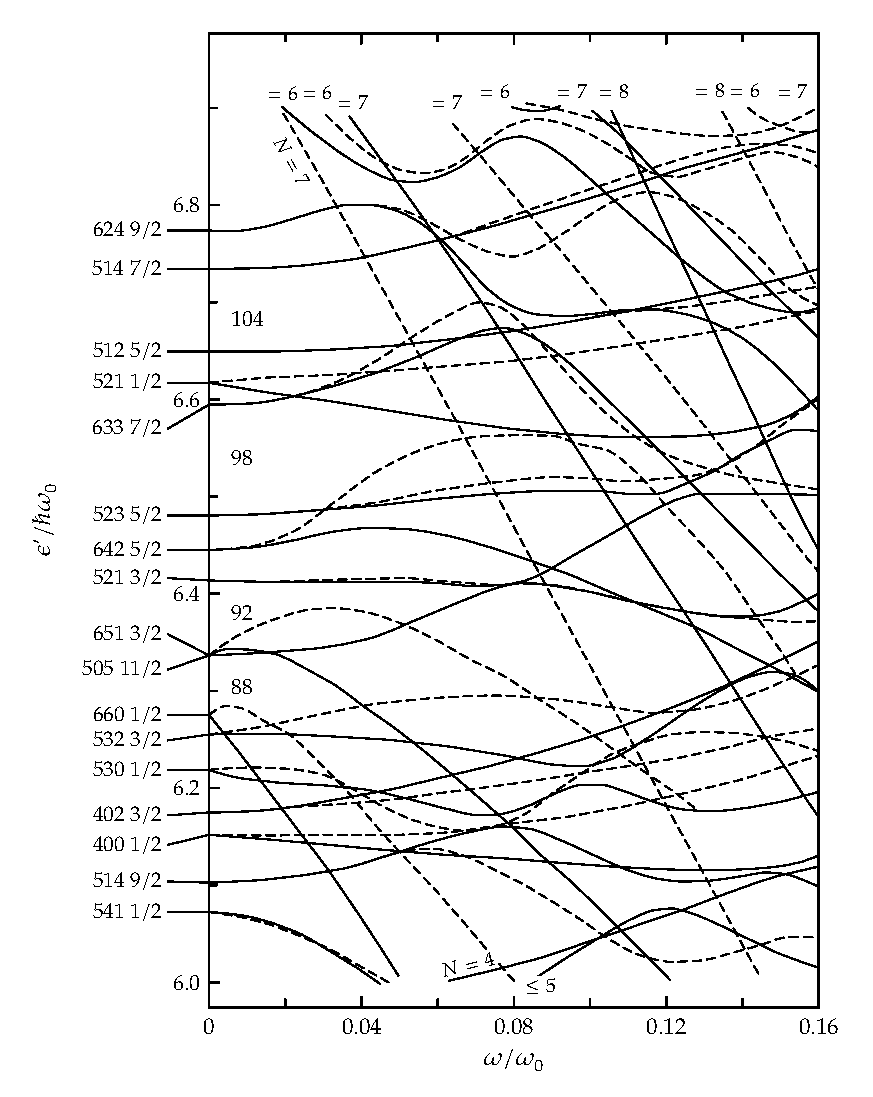
\includegraphics[width=0.75\textwidth]{pictures/3_15}
\par\end{centering}
\caption{\label{fig:3.15}在推引 Nilsson 势中单粒子能级作为 $\omega/\omega_{0}$ 的函数的定性行为。（引自
\cite{RNS78}。）}
\end{figure}


\subsection{高角动量下的形变势能面}

正如我们在 2.9 节中已经讨论过的，纯 Nilsson 模型既不能用于计算总能量，也不能用于计算大形变下的势能面形状，因为在该模型中能量的平均部分没有得到适宜的重现。因此，我们在此模型中仅计算形变能量的振荡部分（壳修正），并将光滑部分替换为相同形变下的液滴能量。

以同样的方式，我们可以计算在固定角动量 $I$ 下能量曲面作为形变的函数。对于椭球形状{[}由参数 $\beta$ 与 $\gamma$
表征，式 (1.88){]}，总能量由下式给出：

\begin{equation}
E(\beta,\gamma,I)=E_{\text{LDM}}(\beta,\gamma,I)+E_{\text{sh}}(\beta,\gamma,I)-\tilde{E}_{\text{sh}}(\beta,\gamma,I)\label{eq:3.123}
\end{equation}
此处 $E_{\text{LDM}}$ 是具有刚体转动惯量 $\mathcal{J}_{\text{rig}}(\beta,\gamma)$
的转动椭球的形变能，因为人们假定在高角动量下对关联可以忽略\footnote{事实上，级联 $\gamma$ 射线的重数测量表明，原子核在高自旋值下确实达到了刚体转动惯量 \cite{SBC76}。}。$E_{\text{sh}}$
是壳模型能量，通过对单粒子能量求和得到。$\tilde{E}_{\text{sh}}$ 是其平均部分，通过适宜的平滑程序算出（参见
2.9 节）。

存在两种途径从转动参考系中形变单粒子势的对角化导出这些物理量：或者在恒定频率 $\omega$ 下开展工作 \cite{NPF76}，或者在恒定角动量
$I$ 下开展工作 \cite{ALL76}。如果使用形变 Woods-Saxon 势（其平均转动惯量非常接近刚体值\footnote{Nilsson 势 (2.89) 中的 $\boldsymbol{l}^{2}$ 项是非局域的并对有效质量产生贡献。它给出的平均转动惯量比刚体值大约大
30–40\% \cite{Ty70,Ty71,BR71b,Je73}。人们曾采用定标程序来补偿这一效应 \cite{NTP77}。} \cite{BJ76b,NTP77}），这两种方法的结果完全一致。

若干研究小组沿着这一思路在周期表的许多区域展开了深入调查 \cite{BLL75,NP75,NPF76,ALL76,FDG76,NTP77}。在定性上他们发现了极为类似的结果：
\begin{enumerate}
\item[(i)] 对于稀土区开端的球形或弱形变核，其行为类似于经典液滴（图 1.18）：直到角动量 $I=50-70\,\hbar$，它们保持为扁椭球并绕对称轴旋转。在这一区域，转动是非集体的，人们预期出现晕阱（参见
3.4.7 节）。对于更高的 $I$ 值，它们迅速转变为三轴和长椭球形变（Jacobi 形状，参见 1.7 节）。这一转变对应于角动量的急剧剧增（“巨回弯”，giant
backbending），如\ref{fig:3.16} 所示。最终原子核发生裂变。
\item[(ii)] 稀土区中部的原子核在低 $I$ 值下从长椭球形状出发，并绕垂直于对称轴的轴旋转。随着转动的加剧，Coriolis 力使粒子顺排并驱动原子核走向非对称形状（三轴形变）。在许多计算中，人们甚至在
$I\sim50-70\,\hbar$ 处发现了向扁椭球形状的转变\footnote{在基于 Woods-Saxon 势的计算中 \cite{NTP77}，原子核不会达到如此极端的三轴形变，并且在尚未达到扁椭球形状之前就已经发生裂变。}，如\ref{fig:3.17}
所示。在极高角动量下，原子核再次变为三轴形变，并最终发生裂变。
\end{enumerate}
\begin{figure}[H]
\begin{centering}
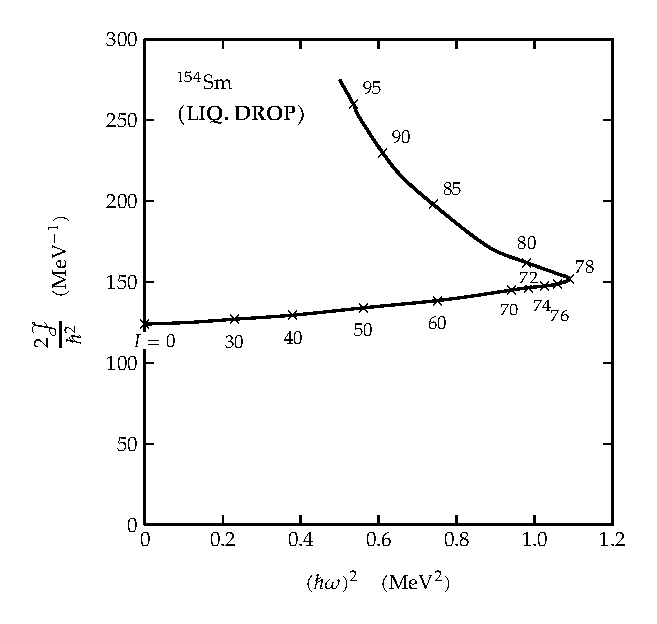
\includegraphics[width=0.75\textwidth]{pictures/3_16}
\par\end{centering}
\caption{\label{fig:3.16}根据转动液滴模型绘制的 $^{154}\text{Sm}$ 晕谱的回弯图。（引自 \cite{ALL76}。）}
\end{figure}

\begin{figure}[H]
\begin{centering}
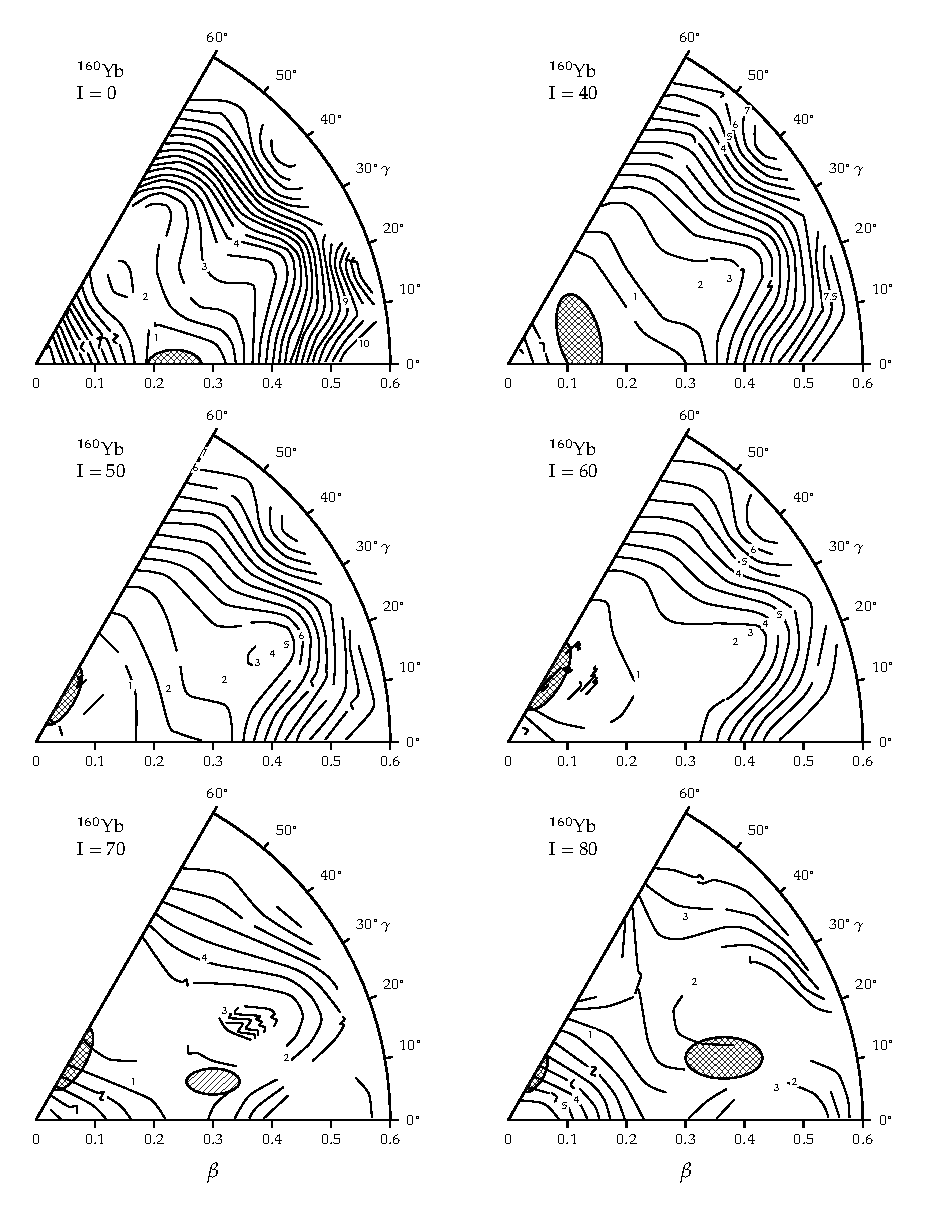
\includegraphics[width=0.75\textwidth]{pictures/3_17}
\par\end{centering}
\caption{\label{fig:3.17}计入壳修正后 $^{160}\text{Yb}$ 在 $(\beta,\gamma)$ 平面内的势能面随角动量的变化关系。（引自
\cite{ALL76}。请注意这些作者将 Hill-Wheeler 坐标 $\gamma$ 替换为 $-\gamma$。）}
\end{figure}

我们想在总结本小节时指出，此类计算仅能给出核多体系统在如此高角动量下行为的定性印象。只有对于极低激发能以及具有深势阱极小值的势能面，我们才能预期原子核具有确定的形变。一般而言，原子核将围绕这些极小值进行量子力学零点涨落，这应当由动力学理论予以描述（例如参见第
10 章）。

\subsection{绕对称轴的转动}

正如我们在前面几小节中所见，在元素周期表中存在一些区域，其中的原子核呈现绕对称轴“转动”。这尤其发生在每个主壳层的开端与末端。在每个壳层的开端，只有少数几个粒子位于或多或少为球形的核心之外。为了产生巨大的角动量，它们必须全部沿转动轴（$x$
轴）顺排；也就是说从经典角度来看，这些粒子必须在赤道平面内绕核运行，从而产生扁椭球的密度分布\footnote{在主壳层末端，类似的论据可以应用于空穴。此时我们最终得到绕长椭球密度分布对称轴的转动。在壳层中部存在许多形成长椭球形变的价粒子，通过少数几次顺排过程就极易产生大角动量，而不会对形变造成太剧烈的改变。}。

这种组态显然不是集体转动，因为其中仅涉及少数几个粒子。每一个单粒子波函数都是 $j_{x}$ 具有本征值 $\alpha_{i}$
的本征函数。总角动量沿对称轴方向的分量由下式给出：

\begin{equation}
\langle I_{x}\rangle=\sum^{A}_{i=1}\alpha_{i}\label{eq:3.124}
\end{equation}
为了增加角动量，我们必须改变形变势中的占据方式，将粒子从具有较低（例如负）$\alpha$ 值的能级提升到具有较高（正）$\alpha$
值的能级中。

在形式上，这同样可以通过绕对称轴的推引程序来实现。由于算符 $j_{x}$ 与 $h$ 对易，我们得到“转动参考系”中的单粒子能量：

\begin{equation}
\epsilon_{i}'=\epsilon_{i}-\omega\alpha_{i}\label{eq:3.125}
\end{equation}
其中 $\epsilon_{i}$ 是 $h$ 在非转动参考系中的本征值。作为 $\omega$ 的函数，它们是一组直线（\ref{fig:3.18}a），其斜率由下式给出：

\begin{equation}
\frac{\mathrm{d}\epsilon_{i}'}{\mathrm{d}\omega}=-\alpha_{i}\label{eq:3.126}
\end{equation}
在转动参考系中极小化能量的条件

\begin{equation}
E'=\sum^{A}_{i=1}(\epsilon_{i}-\omega\alpha_{i})\label{eq:3.127}
\end{equation}
保证了人们总是填充最低的能级 $\epsilon_{i}'$。随着频率 $\omega$ 的增加，我们因此获得了阶梯状递增的角动量（\ref{fig:3.18}b）。两阶之间的距离以及台阶的高度由能级
$\epsilon_{i}$ 之间的间距以及角动量数值 $\alpha_{i}$ 决定。因此，角动量随频率 $\omega$
的增加具有统计性的特征。转动惯量 $\mathcal{J}$ 仅在平均意义上被定义（\ref{fig:3.18}b 中的虚线）。

为了对该转动惯量的大小做出估计 \cite{Bo76b}，我们认识到\ref{fig:3.18}a 中的每一条线都具有斜率 $-\alpha_{i}$（取决于
$\alpha$ 的符号而上升或下降）。在 $\omega=0$ 处，能级 $\pm\alpha_{i}$ 全部成对占据，所得的总角动量为零。对于有限的
$\omega$，其中某些具有负 $\alpha$ 值的能级不再被占据，而其他具有正 $\alpha$ 值的下行能级则被重新占据。对于固定的
$\alpha$ 值（例如 $\alpha=1/2$），新占据能级的数目在平均意义上为 $\omega\alpha g(\alpha)$，其中
$g(\alpha)$ 是量子数为 $\alpha$ 的能级密度。因此在平均意义上我们获得角动量：

\begin{equation}
\langle I_{x}\rangle_{\text{av}}=\sum_{i}\alpha_{i}=\int\alpha\cdot\omega\alpha g(\alpha)\,\mathrm{d}\alpha=\omega\sum_{\alpha}\alpha^{2}g(\alpha)\label{eq:3.128}
\end{equation}
以及平均转动惯量：

\begin{equation}
\mathcal{J}_{\text{av}}=\sum_{\alpha}\alpha^{2}g(\alpha)\label{eq:3.129}
\end{equation}
在 Thomas-Fermi 近似下对该量的求值恰好给出刚体转动惯量的值。因此，绕对称轴的转动在整体上表现出与集体转动极其相似的宏观行为，尽管其微观内部结构截然不同。

\begin{figure}[H]
\begin{centering}
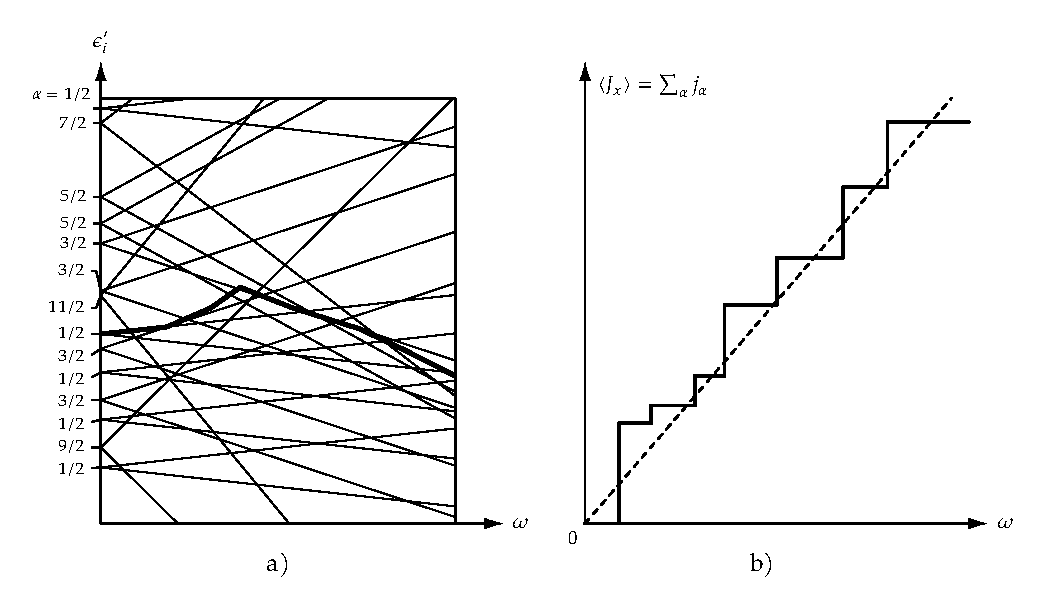
\includegraphics[width=0.75\textwidth]{pictures/3_18}
\par\end{centering}
\caption{\label{fig:3.18}(a) 式 (3.125) 中的本征值 $\epsilon_{i}'$ 作为推引频率的函数的示意图。(b)
随着 $\omega$ 的增加并通过总是占据 (a) 中的最低能级所获得的角动量 $\langle I_{x}\rangle$。}
\end{figure}


\subsection{晕阱}

由于在绕对称轴转动的情形下能级间距具有统计特征，人们预期存在\emph{晕阱}（yrast traps，即高自旋同核异能态）。它们被定义为不能发生快速
$\gamma$ 跃迁的晕态，由 Bohr 和 Mottelson \cite{BM74} 首次预测。

在转动势阱中始终从底部开始填充能级，随着角速度的增加，我们最终会获得角动量跨越若干个单位的跃变（参见\ref{fig:3.18}b）。这在非转动扁椭球形变
Nilsson 势阱的本征值 $\epsilon_{i}$ 作为沿对称轴角动量分量 $\alpha$ 的函数的表示中可以最直观地看清（\ref{fig:3.19}）。对于小形变，我们具有相当纯的
$j$ 组态。处于同一 $j$ 壳层能级的本征值 $\epsilon_{i}$ 近似落在抛物线上{[}参见\ref{eq:3.39}，我们只需将
$\Omega$ 替换为 $\alpha${]}。在扁椭球形变下（$\beta<0$），具有最高 $\alpha$ 值的态（即最大顺排的态）能量最低，因为它们在赤道面内的扁椭球密度分布与核心的扁椭球密度具有最大的重叠。

\begin{figure}[H]
\begin{centering}
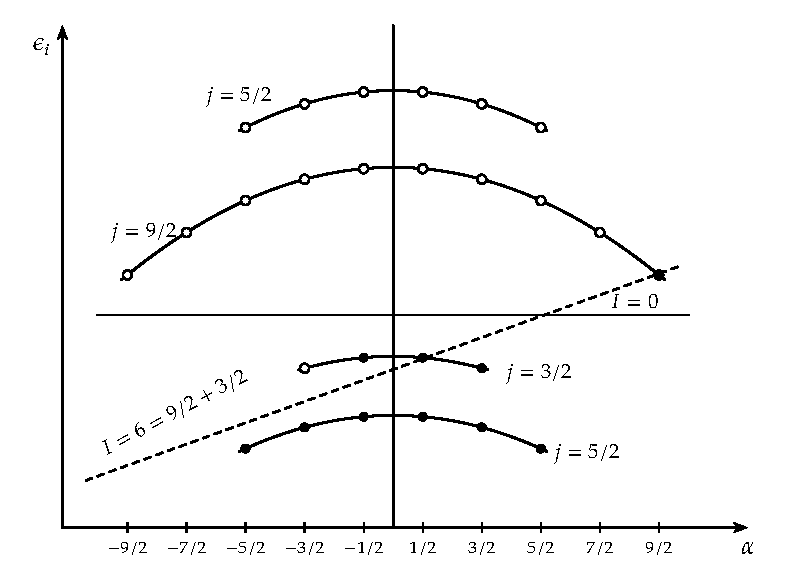
\includegraphics[width=0.75\textwidth]{pictures/3_19}
\par\end{centering}
\caption{\label{fig:3.19}扁椭球形变 Nilsson 势阱中单粒子能量 $\epsilon_{i}$ 作为 $\alpha$（$j_{x}$
的本征值）的函数的示意图，给出了 $I=0$ 处（实线）和 $I=6$ 处（虚线）的 Fermi 面。}
\end{figure}

在 $\omega=0$ 处，Fermi 面是一条水平线，位于其下的所有能级都被占据。在有限的 $\omega$ 值下，根据\ref{eq:3.125}，转动参考系中的
Fermi 面具有斜率 $\omega$。随着 $\omega$ 值的增加，具有负 $\alpha$ 值的能级被腾空，而具有正
$\alpha$ 值的能级被新占据。在\ref{fig:3.19} 中我们展示了发生 6 个单位角动量跃变的情形。晕线上的其余
$I$ 值可以通过构造相对于转动能面的粒子-空穴（ph）组态来获得。这通常伴随着能量的增加。因此，可能会出现晕线不再是 $I$
的单调递增函数的情况，某个具有 $I=I_{0}$ 的能级可能比邻近的 $I=I_{0}-1,I_{0}-2,\dots$ 能级具有更低的能量。此时快速的
$E1,E2,M1$ 或 $M2$ 跃迁（即低多极跃迁；参见附录 B）是不被允许的（所谓\emph{能量自旋阱}，energy
spin traps）。

即使不是这种情况，具有 $I_{0}-1,I_{0}-2$ 的态的内部结构可能与态 $I_{0}$ 的结构截然不同。此时跃迁矩阵元可能非常微小，态
$I_{0}$ 具有极长的寿命（所谓\emph{结构自旋阱}，structure spin traps）。典型的例子是：态 $I_{0}-1$
或 $I_{0}-2$ 只能通过从态 $I_{0}$ 进行 2p-2h 激发才能达到；或者 $\gamma$ 跃迁矩阵元受到单粒子波函数内禀选择定则的阻碍（例如
$l$ 禁戒的 $M1$ 跃迁，参见 2.7.2 节）。

若干研究小组通过在高角动量势能面上寻找绕对称轴转动的范例，并深入研究这些情形下的精细单粒子结构，从理论上探讨了晕阱存在的可能性 \cite{ALL76,CDS77,AK77,DNM77,PFL78,PTF78,AHL78,Ab78,MDN78}。在周期表中已经找到了一些应当预期存在晕阱的区域。它们主要是弱形变核，例如
Te、Ba、Ce、Sm、缺中子稀土同位素以及 Pb 区域的原子核。

在实验方面，人们很早就知道了球形核中具有大角动量和极长寿命的同核异能态。这些态具有相当纯的高 $j$ 壳层组态，对能量更低的其他态不存在低多极的允许
$\gamma$ 跃迁矩阵元。最著名的例子 \cite{PAG62} 是 $^{212}\text{Po}$ 中的 $18^{+}$
同核异能态，其寿命长达 45 秒，由顺排的 $(\pi h^{2}_{9/2})(\nu i_{11/2}g_{9/2})$ 组态构成。

在良好形变核中观测到了另一类高自旋同核异能态，通常称为 $K$-同核异能态，例如 $^{178}\text{Hf}$ 中的 $4\,\text{s}$
和 $31\,\text{y}$ 同核异能态，它们可以解释为 $K^{\pi}=8^{-}$ 和 $K^{\pi}=16^{+}$
的带头，其 $\gamma$ 衰变是 $K$ 禁戒的 \cite{HR68,KL77}。

最后，近年来在轻稀土区发现了由约 20 个相邻原子核组成的长寿命同核异能态“岛” \cite{PBB77}。它们很可能与扁椭球形变和“单粒子”转动相关联
\cite{AHL78}。

邻近 $^{208}\text{Pb}$ 的原子核性质通常是在带有剩余相互作用和适当角动量耦合技术的球形壳模型框架下进行研究的。由于这些组态相当纯净，此类计算能够以非凡的精度解释所测得的激发能
\cite{BBH77}。

在这一物理图像中，顺排的高自旋组态具有如此长寿命的物理原因与我们在绕对称轴转动模型中所解释的完全相同：两个自旋顺排的核子获得能量，是因为对于具有大空间重叠的波函数而言它们的剩余相互作用最大\footnote{该效应被称为 MONA 效应（通过顺排实现核波函数的最大重叠，Maximal Overlap of the Nuclear wave
function by Alignment \cite{FPD76}）。}（参见 4.4.8 节）。因此，这些高自旋能级的能量低于具有较小 $I$ 值的相邻态，快速 $\gamma$ 跃迁受到禁戒。在通过绕对称轴转动的平均场方法对这些核的描述中，相同的效应表现为（正如在\ref{fig:3.18}
中所讨论的）：具有最大 $\alpha$ 值和扁椭球密度分布的顺排能级，因其与扁椭球核心具有巨大的空间重叠，在能量上被大幅向下拉低。

这两种方法——基于角动量耦合技术的球形基底壳模型计算，以及略微形变势阱中的 cranking 计算——无疑是很难进行直接比较的。只要人们能够假定球形核心是惰性的，球形壳模型无疑要优秀得多（尽管它需要付出更多的计算努力），否则人们就必须考虑多粒子-多空穴组态。因此它仅限于幻数核的极其紧邻的区域。在另一方面，cranking
模型通过形变势阱来处理剩余相互作用，因而在广泛的原子核中极易处理。然而它仅允许给出非常定性的预言，因为它破坏了角动量守恒，并且仅在具有垂直于对称轴转动的良好形变核区域才具有微观推导基础（参见
11.4 节）。
